%% ------------------------------------------------------------------
%%  main_timc_revised.tex
%%
%%  Revision of "RBF-ESO Backstepping Control for Multi-UAV Cooperative Payload
%%  Transportation" aligned with the revision-branch code (commit 9339ec5) and
%%  with TIMC_论文修改清单.md.
%%
%%  What changed relative to the submitted manuscript (see README_revised.md):
%%    - RBF: 2-D per-channel features, 5 nodes, one shared basis for output and
%%      update, fixed gain + leakage + closed-ball projection (dead zone removed)
%%    - ESO: driven by the applied wrench F_in/M_in, prediction model contains
%%      gravity and the RBF output, Euler-angle acceleration mapping, 18 states
%%    - Control law: -K0 e_p retained, moments mapped through J0*T^-1
%%    - One common parameter set; takeoff phase removed; 20% evaluation window
%%    - Metrics: geodesic rotation-angle error, tension, allocation residual,
%%      failure criterion; new random-disturbance experiment and numeric tables
%%    - Claims narrowed (ESO dominant, RBF marginal)
%%
%%  Compile: pdflatex main_timc_revised (twice), needs sagej.cls and figures/.
%% ------------------------------------------------------------------
\documentclass[Review,sageh,times]{sagej}

\makeatletter
\@ifpackageloaded{amsmath}{}{\usepackage{amsmath}}
\@ifpackageloaded{amssymb}{}{\usepackage{amssymb}}
\@ifpackageloaded{graphicx}{}{\usepackage{graphicx}}
\@ifpackageloaded{natbib}{}{\usepackage{natbib}}
\makeatother

\usepackage{url}
\usepackage{moreverb}

\graphicspath{{figures/}}

\begin{document}

\title{RBF-ESO Backstepping Control for Multi-UAV Cooperative Payload Transportation}

\author{
Kangkai Li\,\affilnum{1},
Qicheng Wang\,\affilnum{1},
Fan Zhou\,\affilnum{1} and
Jian Sun\,\affilnum{1}
}

\affiliation{\affilnum{1}Xi'an Jiaotong University, Xi'an, China}

\corrauth{Jian Sun, Xi'an Jiaotong University, Xi'an, China.}

\email{sunjian10@xjtu.edu.cn}

\runninghead{Li et al.}

\begin{abstract}
Cooperative payload transportation with multiple unmanned aerial
vehicles (UAVs) is challenging because the payload dynamics are
strongly coupled with cable constraints, nonlinear rotational motion,
allocation errors, and external disturbances. This paper presents a
payload-level RBF-ESO backstepping framework in which the RBF output is
placed inside the ESO prediction model, so that the observer estimates
the residual that remains after learning instead of a separately defined
disturbance. One common parameter set is frozen for every configuration,
and the evidence is organised as a backstepping-family ablation together
with a mass/inertia mismatch sweep, an unmodeled quadratic drag, and a
band-limited non-periodic disturbance experiment. Across these conditions
the ESO-only configuration accounts for most of the error reduction
(about thirteen times relative to plain backstepping under the periodic
disturbance and about eight times under the random one), whereas the
additional RBF term contributes a consistent but modest 6--10\%. The
ordering of the four configurations is preserved under every disturbance
class tested. The paper therefore bounds the role that can be attributed
to each module rather than claiming that the network learns the unmodeled
dynamics.
\end{abstract}

\keywords{multi-UAV cooperative transportation; payload transportation;
backstepping control; RBF neural network; extended state observer;
non-periodic disturbance; ablation}

\def\startpage{2}
\def\volumeyear{2026}

\maketitle

% ==================================================================
\section*{Introduction}
% ==================================================================

UAV technology has developed rapidly in recent years and is now
widely used in aerial imaging, agriculture, industry, and material delivery.
Recently, increasing attention has been directed toward multi-UAV
systems. Compared with single-UAV platforms, multi-UAV cooperative
systems provide higher payload capacity, greater flexibility, and improved
fault tolerance. Among these applications, multi-UAV cooperative
payload transportation has attracted significant interest due to its potential
for transporting heavy and large-sized materials
\citep{fink2011,lee2013c,estevez2024}.

However, cooperative payload transportation remains a challenging
problem in aerial robotics. The presence of flexible cables, coupled motion
constraints, and strong interactions among multiple UAVs and the payload
leads to a high-dimensional, nonlinear, and tightly coupled dynamical
system. In practice, these couplings introduce significant difficulties in
both controller design and stability analysis, especially when precise
trajectory tracking and attitude regulation are required simultaneously
\citep{goodarzi2015,sreenath2013,lee2018}. Although a
complete geometric dynamic model has been established in prior work
\citep{lee2013a,lee2014}, achieving robust and high-accuracy control
under external disturbances, parameter uncertainties, and unmodeled
dynamics is still nontrivial. Therefore, developing control strategies that
combine accurate modeling with strong disturbance-rejection capability
remains an important research direction for cooperative multi-UAV
payload transportation.

To address these challenges, a variety of control strategies have been
developed in the literature. Nonlinear methods, such as backstepping
and sliding-mode control, have been widely adopted for UAV systems
because of their ability to handle strong nonlinearities
\citep{bouabdallah2005,madani2008,thanh2022}.
Nevertheless, these approaches often depend on relatively accurate system
models, and their performance can degrade when significant parameter
uncertainties and unmodeled dynamics are present. To mitigate these
limitations, adaptive control schemes and neural-network-based methods
have been introduced to approximate unknown dynamics online
\citep{sanner1992,park1991,shen2021}. In
addition, ESO and ADRC methods provide a practical observer-based
route for estimating lumped disturbances and improving robustness
\citep{han2009,gao2003,madonski2015,wang2022}.
These developments motivate the use of learning-based compensation
terms together with robust feedback to improve tracking performance
under modeling uncertainty.

In this paper, we develop an RBF-ESO backstepping controller for
multi-UAV cooperative payload transportation. Backstepping is adopted
as the nominal nonlinear tracking controller because it provides a recursive
error-stabilization structure for the payload translation and attitude
channels. A bank of small RBF networks supplies an additional online
compensation term \citep{broomhead1988,park1991,shen2021}, and an ESO
estimates the lumped residual that remains \emph{after} that compensation
\citep{han2009,madonski2015,gu2022}. The structural point is that the RBF
output enters the ESO prediction model: the observer therefore tracks a
residual that changes while the network learns, instead of estimating a
disturbance that is defined independently of the learning module.

The contribution of this paper is a controlled ablation framework
together with the residual-consistent architecture it evaluates. The
framework freezes one common parameter set for all variants, reports the
marginal value of each module, and states explicitly which conclusions
the numerical evidence does and does not support. The evidence covers a
periodic multi-harmonic disturbance, a band-limited non-periodic
disturbance over five fixed seeds, mass and inertia mismatches from
$0.5$ to $1.5$ times the nominal values, and an unmodeled quadratic drag
reaching about $74\%$ of the payload weight. The resulting statement is
deliberately narrow: the observer carries most of the compensation, the
learning module adds a consistent but modest margin, and the ordering of
the four configurations is preserved across the disturbance classes tested.

% ==================================================================
\section*{System Modeling}
% ==================================================================

The dynamic model used in this paper is based on the geometric
formulation proposed by Lee et al.\ for multiple quadrotor UAVs
transporting a cable-suspended rigid body \citep{lee2013a,lee2013c}. In that
framework, a cooperative aerial transportation system consists of $N$
quadrotors carrying a rigid payload through massless, taut, inextensible
cables. The payload dynamics and individual quadrotor dynamics are
derived separately and are coupled through kinematic constraints.

\subsection*{Coordinate Frames and State Representation}

We define three primary coordinate frames:

\emph{Inertial Frame (I)} A fixed Earth frame defined by basis vectors
$\{\mathbf{e}_1,\mathbf{e}_2,\mathbf{e}_3\}$, with $\mathbf{e}_3=[0,0,1]^T$ pointing
\textbf{upward}; gravity therefore enters the translational dynamics as
$-g\mathbf{e}_3$, which is the convention used consistently in the model,
the controller, and the implementation.

\emph{Payload Body Frame (L)} Attached to the payload center of mass (CoM),
with orientation $\mathbf{R}_L\in SO(3)$ relative to $I$.

\emph{Quadrotor Body Frame (B$_i$)} Attached to the CoM of the $i$-th quadrotor
($i=1\ldots N$), with orientation $\mathbf{R}_i\in SO(3)$ relative to $I$.

For both the payload and each quadrotor, the dynamic variables are
position $\mathbf{p}$, linear velocity $\mathbf{v}$, attitude matrix $\mathbf{R}$, and angular velocity $\boldsymbol{\Omega}$.
Here, $\mathbf{p}$ and $\mathbf{v}$ are expressed in the inertial frame, $\mathbf{R}\in SO(3)$ denotes
attitude, and $\boldsymbol{\Omega}$ is expressed in the corresponding body frame. Subscripts
denote object indices: $L$ for the payload, $i$ for the $i$-th quadrotor (or cable),
and $ext$ for external disturbances.

\begin{figure}[t]
\centering
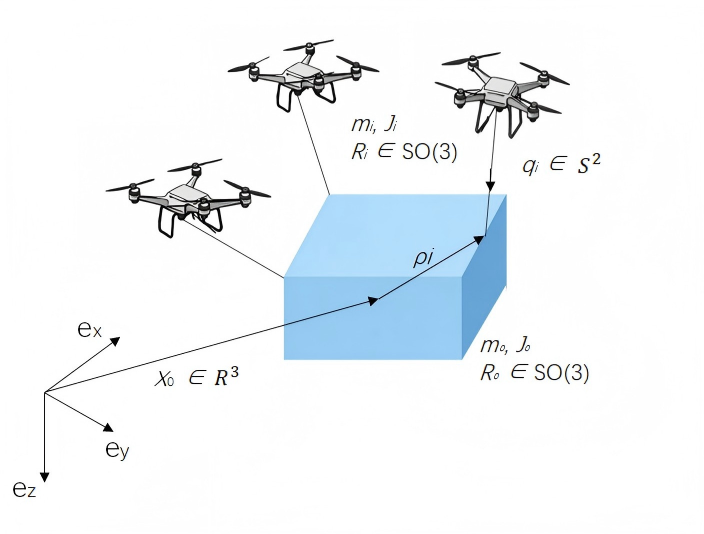
\includegraphics[width=0.97\textwidth]{fig1_geometry}
\caption{The UAVs and payload geometric structure.}
\label{fig:geometry}
\end{figure}

\subsection*{Kinematic Constraints}

The payload is connected to the $i$-th quadrotor by a taut, inextensible cable
of length $l_i$. Let $\boldsymbol{\rho}_i$ be the vector of the connection point on the load in the
$L$ frame, then the geometric relationship follows the equation below.
\begin{equation}
\mathbf{p}_i = \mathbf{p}_L + \mathbf{R}_L\boldsymbol{\rho}_i - l_i\mathbf{q}_i
\label{eq:kinconstraint}
\end{equation}
where $\mathbf{q}_i\in S^2$ is the unit vector representing the cable direction, pointing
from the quadrotor to the payload.

Differentiating with respect to time yields the velocity relationship
\begin{equation}
\mathbf{v}_i = \mathbf{v}_L + \mathbf{R}_L(\boldsymbol{\Omega}_L\times\boldsymbol{\rho}_i) - l_i\boldsymbol{\omega}_i\times\mathbf{q}_i,
\label{eq:velconstraint}
\end{equation}
where the cable angular velocity satisfies $\dot{\mathbf{q}}_i=\boldsymbol{\omega}_i\times\mathbf{q}_i$.

\subsection*{Payload Dynamics}

We consider a 6-DOF rigid body with mass $m_L$ and inertia tensor $\mathbf{J}_L$, and
derive the equations of motion using the Newton--Euler method.

\emph{Translational Dynamics} The total force acting on the payload is
composed of gravity, the tension forces $\mathbf{T}_i$ from all $N$ cables, and an
external disturbance force $\mathbf{f}_{ext}$:
\begin{equation}
m_L\dot{\mathbf{v}}_L = -m_L g\mathbf{e}_3 + \sum_{i=1}^{N}\mathbf{T}_i + \mathbf{f}_{ext},
\label{eq:paytransl}
\end{equation}
where $\mathbf{T}_i=-\mu_i\mathbf{q}_i$ is the cable force and $\mu_i>0$ is the
corresponding tension magnitude, so that the signed tension indicator used
later is $T_i=-\mathbf{q}_i^{T}\boldsymbol{\mu}_i$ with $\boldsymbol{\mu}_i$ the force
actually applied by the $i$-th cable (the signed indicator is defined in ``Control Allocation and Cable Force Generation'').

\emph{Rotational Dynamics} The rotational motion is driven by the moments
generated by the cable forces applied at lever arms $\boldsymbol{\rho}_i$:
\begin{equation}
\mathbf{J}_L\dot{\boldsymbol{\Omega}}_L = -\boldsymbol{\Omega}_L\times(\mathbf{J}_L\boldsymbol{\Omega}_L)
+ \sum_{i=1}^{N}\boldsymbol{\rho}_i\times(\mathbf{R}_L^{T}\mathbf{T}_i) + \mathbf{J}_L\mathbf{d}_R,
\label{eq:payrot}
\end{equation}
where $\mathbf{d}_R\in\mathbb{R}^3$ is an external \emph{angular acceleration}
(rad/s$^2$), which is how the disturbance is injected in the implementation;
an equivalent disturbance moment is $\mathbf{J}_L\mathbf{d}_R$.

\subsection*{Quadrotor Dynamics}

Each quadrotor is treated as an independent rigid body subject to its own
thrust, gravity, and the reaction force from the cable tension ($-\mathbf{T}_i$).

\emph{Translational Dynamics}
\begin{equation}
m_i\dot{\mathbf{v}}_i = -m_i g\mathbf{e}_3 - f_i\mathbf{R}_i\mathbf{e}_3 - \mathbf{T}_i,
\label{eq:quadtransl}
\end{equation}
where $f_i$ is the total scalar thrust generated by the $i$-th quadrotor rotors,
and $-\mathbf{R}_i\mathbf{e}_3$ represents the thrust direction in the inertial frame.

\emph{Rotational Dynamics}
\begin{equation}
\mathbf{J}_i\dot{\boldsymbol{\Omega}}_i = -\boldsymbol{\Omega}_i\times(\mathbf{J}_i\boldsymbol{\Omega}_i) + \boldsymbol{\tau}_i,
\label{eq:quadrot}
\end{equation}
where $\boldsymbol{\tau}_i=[\tau_\phi,\tau_\theta,\tau_\psi]^T$ are the control torques in the body frame.

% ==================================================================
\section*{Hierarchical Control Design}
% ==================================================================

To address uncertainties in payload dynamics and external disturbances,
we propose an adaptive robust control scheme that integrates backstepping
control, radial basis function (RBF) neural-network approximation, and
extended state observer (ESO) disturbance estimation while following the
geometric payload-transport control framework in \citep{lee2013a,lee2018}.
The backstepping component generates the nominal payload force
and moment commands, the RBF bank compensates part of the unmodeled
nonlinear dynamics \citep{sanner1992,park1991}, and the ESO estimates the
residual that the network does not capture \citep{han2009,madonski2015}.

The overall signal flow is shown in Fig.~\ref{fig:pipeline}. The payload tracking errors are
processed by the nominal backstepping structure, while the RBF and ESO
modules provide online compensation. The resulting payload-level force and
moment commands are distributed through the cable-force allocation layer
and converted into executable quadrotor thrust and attitude commands. Note
that the observer is driven by the wrench that the allocation layer actually
applies, not by the commanded wrench.

\begin{figure}[t]
\centering
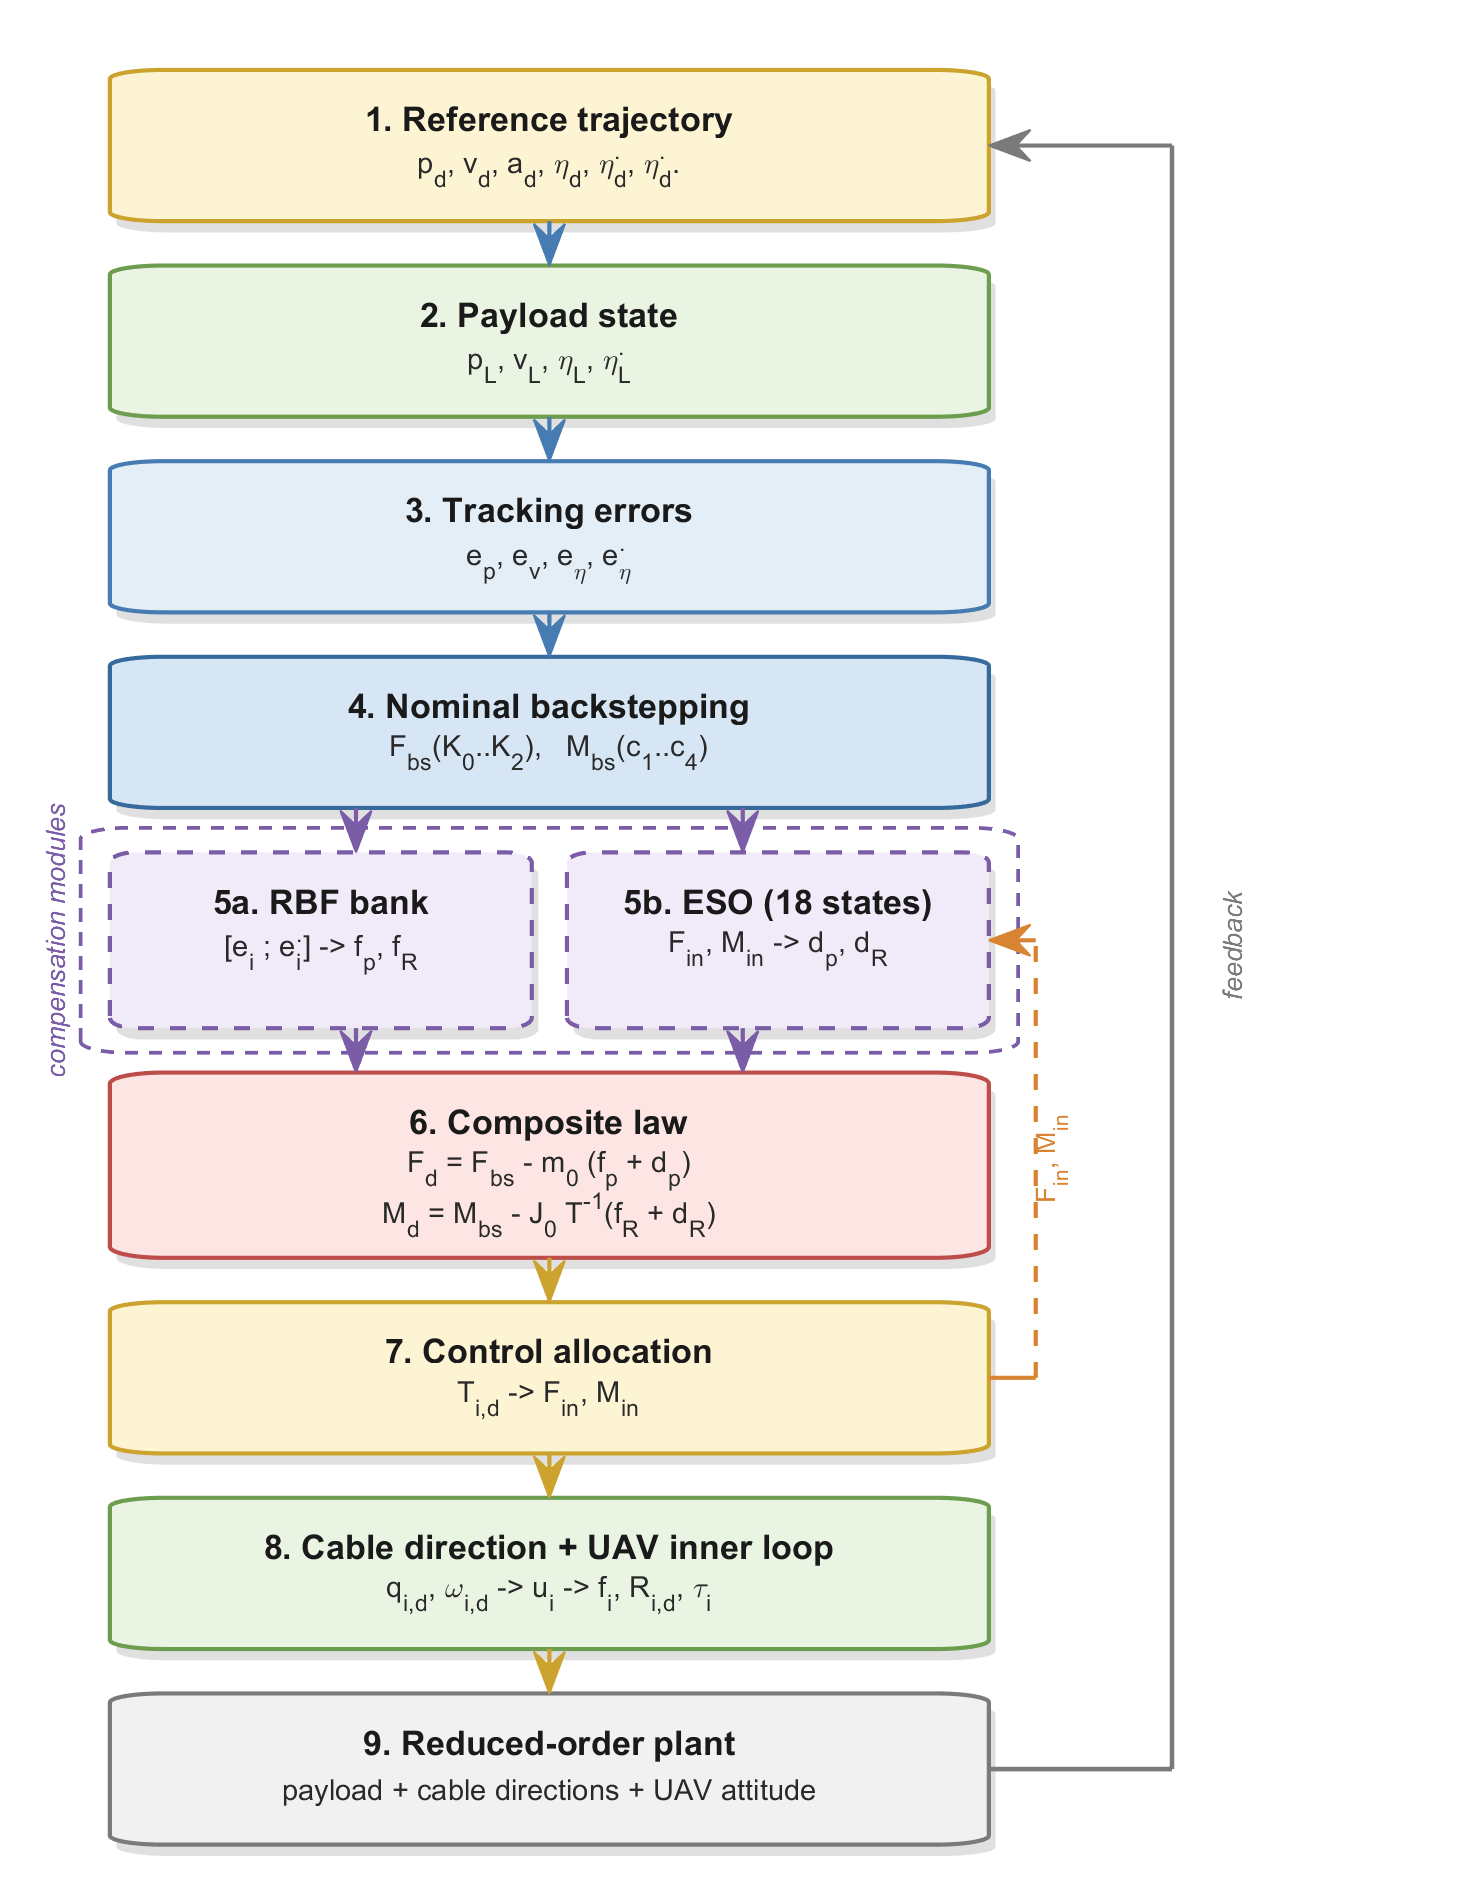
\includegraphics[width=\textwidth]{fig2_pipeline}
\caption{Pipeline of the proposed RBF-ESO backstepping control framework. The ESO
prediction model contains the RBF output and is driven by the applied wrench
$(\mathbf{F}_{in},\mathbf{M}_{in})$ returned by the allocation layer.}
\label{fig:pipeline}
\end{figure}

\subsection*{State and Error Definitions}

The payload translational state is described by the position $\mathbf{p}_L\in\mathbb{R}^3$ and
linear velocity $\mathbf{v}_L\in\mathbb{R}^3$, with desired trajectories $\mathbf{p}_{L,d}$ and $\mathbf{v}_{L,d}$. The
payload attitude can be equivalently represented by the rotation matrix
$\mathbf{R}_L\in SO(3)$ for geometric modeling, while the implemented
controller uses ZYX Euler angles. Let
\begin{equation}
\boldsymbol{\Theta}_L =
\begin{bmatrix}
\phi_L\\ \theta_L\\ \psi_L
\end{bmatrix},
\qquad
\boldsymbol{\Theta}_{L,d} =
\begin{bmatrix}
\phi_{L,d}\\ \theta_{L,d}\\ \psi_{L,d}
\end{bmatrix},
\label{eq:eulerdef}
\end{equation}
denote the current and desired Euler-angle vectors, and let
$\dot{\boldsymbol{\Theta}}_L=\mathbf{T}(\boldsymbol{\Theta}_L)\boldsymbol{\Omega}_L$
be the Euler-angle rate, with $\mathbf{T}(\cdot)$ the ZYX kinematic matrix and
$\dot{\mathbf{T}}$ its time derivative. The tracking errors used in the controller are
\begin{equation}
\begin{aligned}
\mathbf{e}_{p_L} &= \mathbf{p}_L - \mathbf{p}_{L,d},
& \mathbf{e}_{v_L} &= \mathbf{v}_L - \dot{\mathbf{p}}_{L,d},\\
\mathbf{e}_{\Theta_L} &= \mathrm{wrap}(\boldsymbol{\Theta}_L - \boldsymbol{\Theta}_{L,d}),
& \mathbf{e}_{\dot\Theta_L} &= \dot{\boldsymbol{\Theta}}_L - \dot{\boldsymbol{\Theta}}_{L,d},
\end{aligned}
\label{eq:errors}
\end{equation}
where $\mathrm{wrap}(\cdot)$ maps each angle difference to $(-\pi,\pi]$ so that a
crossing of the $\pm\pi$ boundary does not produce a spurious error.

The RBF banks are \emph{channel-wise}: channel $i$ receives its own
two-dimensional feature vector
\begin{equation}
\boldsymbol{\xi}_i =
\begin{bmatrix}
e_i\\ \dot{e}_i
\end{bmatrix}
\in\mathbb{R}^2,
\qquad i=1,\ldots,6,
\label{eq:rbfinput}
\end{equation}
where $e_i$, $i=1,2,3$, are the components of $\mathbf{e}_{p_L}$ with
$\dot e_i$ the corresponding velocity error, and $e_i$, $i=4,5,6$, are the
components of $\mathbf{e}_{\Theta_L}$ with $\dot e_i$ the corresponding Euler-rate
error. Using a two-dimensional feature per channel keeps the number of
adaptive parameters at $6\times5=30$ while avoiding the information
collapse of a single shared six-dimensional input.

\subsection*{RBF Neural Network Approximation}

RBF networks are widely used for nonlinear function approximation
because Gaussian basis functions yield a linearly parameterized
approximator with universal approximation capability
\citep{broomhead1988,park1991}. In this work the approximation is not
implemented as a single global network. Instead, six scalar Gaussian RBF
networks are used in parallel: three for payload translation and three for
payload attitude. Each channel has its own input vector (\ref{eq:rbfinput}),
its own basis, and its own adaptive weight vector; the total number of
adaptive parameters is therefore $6\times5=30$.

Before the basis functions are evaluated, each channel is scaled by a fixed
diagonal matrix so that both entries of $\boldsymbol{\xi}_i$ have comparable
magnitude:
\begin{equation}
\mathbf{x}_i = \mathbf{S}_i^{-1}\boldsymbol{\xi}_i,
\qquad
\mathbf{S}_i =
\begin{cases}
\mathrm{diag}(0.5\ \mathrm{m},\,0.5\ \mathrm{m/s}), & i=1,2,3,\\[1mm]
\mathrm{diag}(0.10\ \mathrm{rad},\,0.50\ \mathrm{rad/s}), & i=4,5,6.
\end{cases}
\label{eq:scaling}
\end{equation}
The channel-wise structure is illustrated in Fig.~\ref{fig:rbf}.

\begin{figure}[t]
\centering
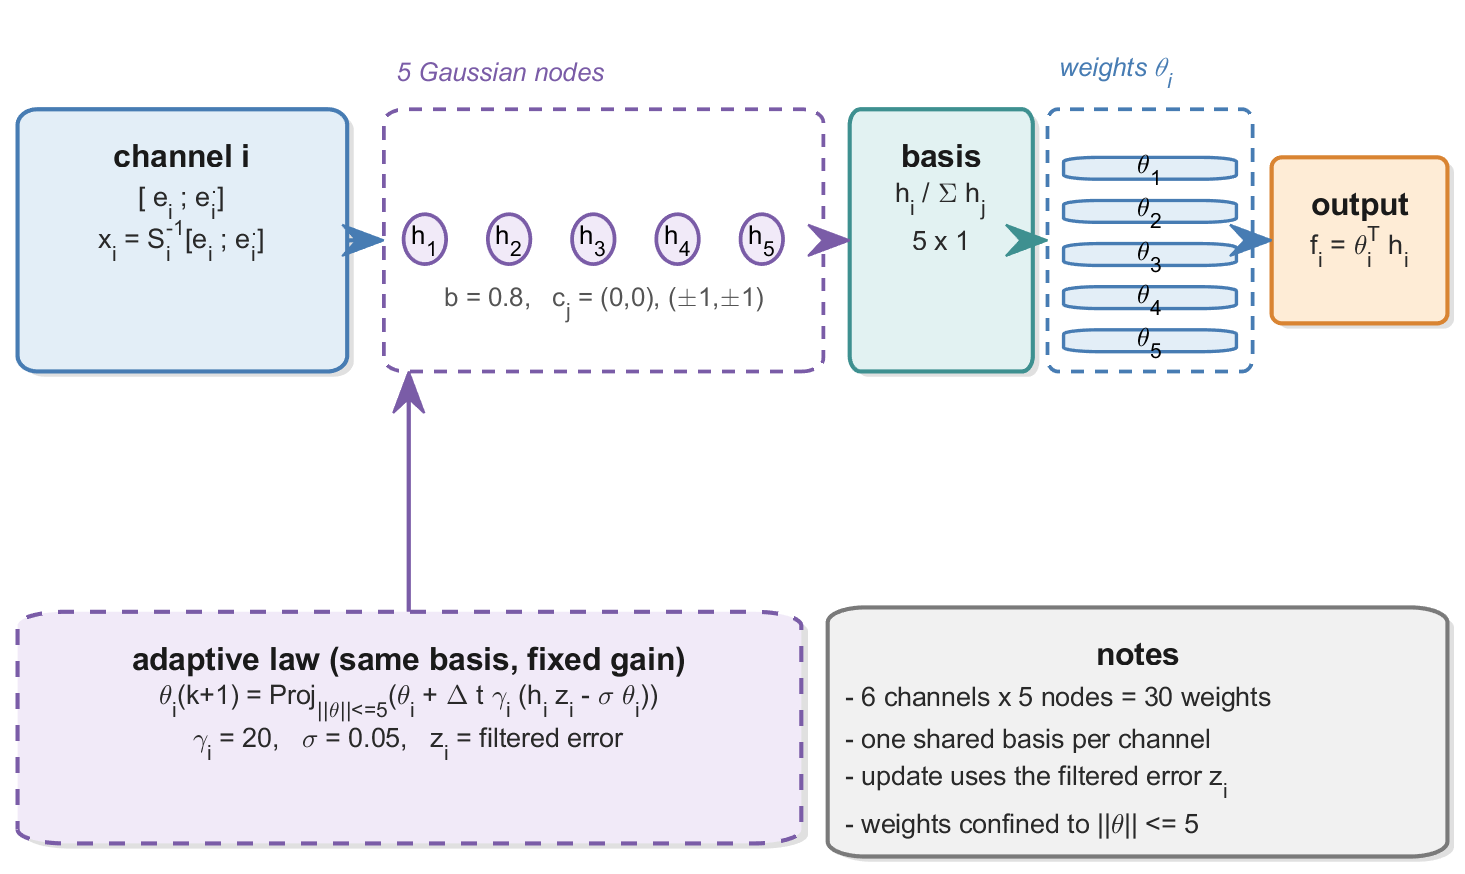
\includegraphics[width=\textwidth]{fig3_rbf}
\caption{Channel-wise RBF network used for payload uncertainty approximation.
One channel is shown; the same five-node structure is repeated for the three
translation and three attitude channels, and the output and the adaptation
update share the same normalised basis.}
\label{fig:rbf}
\end{figure}

For the $j$-th basis node of channel $i$, the Gaussian activation is
\begin{equation}
h_{i,j} = \exp\left(-\frac{\|\mathbf{x}_i - \mathbf{c}_j\|^2}{2b^2}\right),
\qquad j=1,\ldots,5,
\label{eq:gauss}
\end{equation}
with a common width $b=0.8$ and five centres placed at the origin and at the
four corners of the normalised plane,
$\mathbf{c}_j\in\{(0,0),(\pm1,\pm1)\}$. The centres therefore cover the
region in which the scaled errors are expected to evolve, and they are not
obtained by replicating a scalar into several dimensions. The basis is
normalised channel-wise,
\begin{equation}
\bar{\mathbf{h}}_i(\mathbf{x}_i) =
\frac{\mathbf{h}_i(\mathbf{x}_i)}{\sum_{j=1}^{5}h_{i,j}(\mathbf{x}_i)},
\qquad
\mathbf{h}_i =
\begin{bmatrix}
h_{i,1} & \cdots & h_{i,5}
\end{bmatrix}^{T},
\label{eq:normbasis}
\end{equation}
where the denominator is replaced by a small positive constant when it
becomes negligible. The same normalised basis is used for the network
output and for the weight update.

For the translational channels, let $\hat{\boldsymbol{\theta}}_{p,k}\in\mathbb{R}^5$,
$k=1,2,3$, denote the adaptive weight vectors of the $x$-, $y$-, and
$z$-directions. The RBF outputs are
\begin{equation}
\hat{f}_{p,k} = \hat{\boldsymbol{\theta}}_{p,k}^{T}\bar{\mathbf{h}}_k,
\qquad k=1,2,3,
\label{eq:rbfpos}
\end{equation}
stacked as
\begin{equation}
\hat{\mathbf{f}}_p =
\begin{bmatrix}
\hat{f}_{p,1} & \hat{f}_{p,2} & \hat{f}_{p,3}
\end{bmatrix}^{T}.
\label{eq:rbfposvec}
\end{equation}
In the force controller $\hat{\mathbf{f}}_p$ is interpreted as an estimate of
acceleration-level uncertainty in the payload translational dynamics, which
is why it appears multiplied by the nominal payload mass $m_0$.

Similarly, for the attitude channels, let $\hat{\boldsymbol{\theta}}_{R,k}\in\mathbb{R}^5$,
$k=1,2,3$, denote the weights for roll, pitch, and yaw. The outputs and the
stacked vector are
\begin{equation}
\hat{f}_{R,k} = \hat{\boldsymbol{\theta}}_{R,k}^{T}\bar{\mathbf{h}}_{k+3},
\qquad
\hat{\mathbf{f}}_R =
\begin{bmatrix}
\hat{f}_{R,1} & \hat{f}_{R,2} & \hat{f}_{R,3}
\end{bmatrix}^{T},
\label{eq:rbfatt}
\end{equation}
which is an estimate of Euler-angle acceleration and is therefore mapped to
a moment through the same kinematic matrix as the nominal control, see
(\ref{eq:Md}).

The weights are updated online with a channel-wise law that uses the
filtered backstepping error of that channel,
\begin{equation}
\dot{\hat{\boldsymbol{\theta}}}_i =
\gamma_i\left(\bar{\mathbf{h}}_i z_i - \sigma\hat{\boldsymbol{\theta}}_i\right),
\qquad
z_i =
\begin{cases}
e_{v,i} + c_3 e_{p,i}, & i=1,2,3,\\[1mm]
\dot e_{\Theta,i} + c_1 e_{\Theta,i}, & i=4,5,6,
\end{cases}
\label{eq:adaptlaw}
\end{equation}
with a fixed gain $\gamma_i=20$ for all six channels and a leakage
coefficient $\sigma=0.05$. The leakage term bounds the weights in the
absence of persistent excitation; it is not an error dead zone, and no
error-dependent gain scheduling is used. The update is integrated with
forward Euler and projected onto the closed ball of radius $\theta_{\max}=5$,
\begin{equation}
\hat{\boldsymbol{\theta}}_i(k+1) =
\mathrm{Proj}_{\|\hat{\boldsymbol{\theta}}\|\le\theta_{\max}}
\left(
\hat{\boldsymbol{\theta}}_i(k) + \Delta t\,\dot{\hat{\boldsymbol{\theta}}}_i(k)
\right).
\label{eq:proj}
\end{equation}
This projection is the only parameter-protection mechanism retained; no
element-wise saturation and no output limiting are applied, so the model
assumed in the analysis below is the model that is actually implemented.

\subsection*{ESO-Based Residual Estimation}

Even with the RBF term active, model residuals and external disturbances
remain. Let
\begin{equation}
\mathbf{d}_{\mathrm{res}} = \mathbf{f}_{\mathrm{unk}} - \hat{\mathbf{f}}_{\mathrm{RBF}} + \mathbf{d}_{\mathrm{ext}}
\label{eq:residual}
\end{equation}
be the residual that the network does not explain, where
$\mathbf{f}_{\mathrm{unk}}$ collects the unmodeled acceleration-level terms and
$\mathbf{d}_{\mathrm{ext}}$ the external disturbance. The ESO estimates
$\mathbf{d}_{\mathrm{res}}$, not the external disturbance alone; consequently the
RBF parameter error does not enter the analysis twice.

For the translational channel the payload dynamics are written in
acceleration form as
\begin{equation}
\ddot{\mathbf{p}}_L = \frac{\mathbf{F}_{in}}{m_0} - g\mathbf{e}_3
+ \hat{\mathbf{f}}_p + \mathbf{d}_p,
\label{eq:posacc}
\end{equation}
where $\mathbf{F}_{in}$ is the resultant force actually applied by the cables,
$m_0$ the nominal payload mass, and $\mathbf{d}_p$ the translational residual.
Note that $m_0$ appears once: the applied force is divided by the nominal
mass, and gravity is grouped with the known terms. Define the augmented
state $\mathbf{z}_p=[\mathbf{p}_L^{T},\dot{\mathbf{p}}_L^{T},\mathbf{d}_p^{T}]^{T}$ and the
observer
\begin{equation}
\begin{cases}
\dot{\hat{\mathbf{z}}}_{p1} = \hat{\mathbf{z}}_{p2} + \boldsymbol{\beta}_{p1}\left(\mathbf{z}_{p1}-\hat{\mathbf{z}}_{p1}\right),\\[1mm]
\dot{\hat{\mathbf{z}}}_{p2} = \hat{\mathbf{z}}_{p3} + \dfrac{\mathbf{F}_{in}}{m_0} - g\mathbf{e}_3 + \hat{\mathbf{f}}_p
+ \boldsymbol{\beta}_{p2}\left(\mathbf{z}_{p1}-\hat{\mathbf{z}}_{p1}\right),\\[1mm]
\dot{\hat{\mathbf{z}}}_{p3} = \boldsymbol{\beta}_{p3}\left(\mathbf{z}_{p1}-\hat{\mathbf{z}}_{p1}\right),
\end{cases}
\label{eq:esopos}
\end{equation}
where $\mathbf{z}_{p1}=\mathbf{p}_L$, $\mathbf{z}_{p2}=\dot{\mathbf{p}}_L$,
$\mathbf{z}_{p3}=\mathbf{d}_p$, and $\hat{\mathbf{z}}_{p3}$ estimates the residual. The
gains are parameterised by a single bandwidth $\omega_0=50$~rad/s,
\begin{equation}
\boldsymbol{\beta}_{p1}=3\omega_0\mathbf{I}_3,\qquad
\boldsymbol{\beta}_{p2}=3\omega_0^{2}\mathbf{I}_3,\qquad
\boldsymbol{\beta}_{p3}=\omega_0^{3}\mathbf{I}_3 .
\label{eq:esogain}
\end{equation}

For the attitude channel the same construction is applied to the Euler-angle
dynamics. Differentiating $\dot{\boldsymbol{\Theta}}_L=\mathbf{T}\boldsymbol{\Omega}_L$ gives
\begin{equation}
\begin{aligned}
\ddot{\boldsymbol{\Theta}}_L &= \mathbf{f}_{R,0} + \hat{\mathbf{f}}_R + \mathbf{d}_R,\\
\mathbf{f}_{R,0} &:= \mathbf{T}\mathbf{J}_0^{-1}\left(\mathbf{M}_{in}
- \boldsymbol{\Omega}_L\times\mathbf{J}_0\boldsymbol{\Omega}_L\right)
+ \dot{\mathbf{T}}\boldsymbol{\Omega}_L,
\end{aligned}
\label{eq:attacc}
\end{equation}
where $\mathbf{M}_{in}$ is the moment actually applied by the cables and
$\mathbf{d}_R$ the attitude residual. Note that the inertia is not used as a
multiplier of the moment; the Euler-angle acceleration is obtained through
$\mathbf{T}\mathbf{J}_0^{-1}(\cdot)$, which is the map implied by the kinematics. The
observer has the same structure,
\begin{equation}
\begin{cases}
\dot{\hat{\mathbf{z}}}_{\eta1} = \hat{\mathbf{z}}_{\eta2} + \boldsymbol{\beta}_{\eta1}\left(\mathbf{z}_{\eta1}-\hat{\mathbf{z}}_{\eta1}\right),\\[1mm]
\dot{\hat{\mathbf{z}}}_{\eta2} = \hat{\mathbf{z}}_{\eta3} + \mathbf{f}_{R,0} + \hat{\mathbf{f}}_R
+ \boldsymbol{\beta}_{\eta2}\left(\mathbf{z}_{\eta1}-\hat{\mathbf{z}}_{\eta1}\right),\\[1mm]
\dot{\hat{\mathbf{z}}}_{\eta3} = \boldsymbol{\beta}_{\eta3}\left(\mathbf{z}_{\eta1}-\hat{\mathbf{z}}_{\eta1}\right),
\end{cases}
\label{eq:esoatt}
\end{equation}
with $\mathbf{z}_{\eta1}=\boldsymbol{\Theta}_L$ and the same bandwidth
parameterisation. The two blocks give $9+9=18$ observer states in total.

Because the observer is updated with the wrench of the \emph{previous}
interval, the implementation is a discrete-time forward-Euler observer,
\begin{equation}
\hat{\mathbf{z}}(k+1) = \hat{\mathbf{z}}(k) + \Delta t\,
f_{\mathrm{ESO}}\left(\hat{\mathbf{z}}(k),\mathbf{F}_{in}(k-1),\mathbf{M}_{in}(k-1),
\hat{\mathbf{f}}(k)\right),
\label{eq:esodiscrete}
\end{equation}
so that prediction model, measurement, weights, and applied input refer to
the same sampling instants.

\subsection*{Payload Control Law}

The payload-layer controller computes the desired force $\mathbf{F}_d$ in the
inertial frame and the desired moment $\mathbf{M}_d$ in the body frame.

\emph{Translational Control} With the errors of (\ref{eq:errors}), the virtual control
is
\begin{equation}
\boldsymbol{\alpha}_p = -\mathbf{K}_{p1}\mathbf{e}_{p_L} + \dot{\mathbf{p}}_{L,d},
\qquad
\mathbf{z}_p = \mathbf{e}_{v_L} + \mathbf{K}_{p1}\mathbf{e}_{p_L},
\label{eq:alphap}
\end{equation}
and the nominal backstepping force is
\begin{equation}
\mathbf{F}_{d,bs} = m_0\left(-g\mathbf{e}_3 + \ddot{\mathbf{p}}_{L,d}
- \mathbf{K}_{p1}\mathbf{e}_{v_L} - \mathbf{K}_{p0}\mathbf{e}_{p_L}
- \mathbf{K}_{p2}\mathbf{z}_p\right),
\label{eq:Fdbs}
\end{equation}
where $\mathbf{K}_{p1},\mathbf{K}_{p2}\succ0$ are diagonal gain matrices. The term
$-\mathbf{K}_{p0}\mathbf{e}_{p_L}$ with $\mathbf{K}_{p0}=\mathbf{I}_3$ is the unit proportional
gain retained from the original implementation; it is not retuned in this
work. Adding the RBF and residual compensation gives
\begin{equation}
\mathbf{F}_d = \mathbf{F}_{d,bs} - m_0\hat{\mathbf{f}}_p - m_0\hat{\mathbf{z}}_{p3}.
\label{eq:Fd}
\end{equation}

\emph{Rotational Control} With the attitude errors of (\ref{eq:errors}), define
\begin{equation}
\boldsymbol{\alpha}_\eta = -\mathbf{K}_{\eta1}\mathbf{e}_{\Theta_L} + \dot{\boldsymbol{\Theta}}_{L,d},
\qquad
\mathbf{z}_\eta = \mathbf{e}_{\dot\Theta_L} + \mathbf{K}_{\eta1}\mathbf{e}_{\Theta_L}.
\label{eq:alphaeta}
\end{equation}
The nominal Euler-angle acceleration command is
\begin{equation}
\ddot{\boldsymbol{\Theta}}_{c} = \ddot{\boldsymbol{\Theta}}_{L,d}
- \mathbf{K}_{\eta1}\mathbf{e}_{\dot\Theta_L} - \mathbf{e}_{\Theta_L}
- \mathbf{K}_{\eta2}\mathbf{z}_\eta,
\label{eq:etaddot}
\end{equation}
again with the unit proportional term $-\mathbf{e}_{\Theta_L}$ inherited from the
implementation, and the nominal moment follows from the inverse of the
kinematic map in (\ref{eq:attacc}),
\begin{equation}
\mathbf{M}_{d,bs} = \mathbf{J}_0\mathbf{T}^{-1}\left(\ddot{\boldsymbol{\Theta}}_{c}
- \dot{\mathbf{T}}\boldsymbol{\Omega}_L\right) + \boldsymbol{\Omega}_L\times\mathbf{J}_0\boldsymbol{\Omega}_L .
\label{eq:Mdbs}
\end{equation}
The composite moment is
\begin{equation}
\mathbf{M}_d = \mathbf{M}_{d,bs}
- \mathbf{J}_0\mathbf{T}^{-1}\hat{\mathbf{f}}_R
- \mathbf{J}_0\mathbf{T}^{-1}\hat{\mathbf{z}}_{\eta3},
\label{eq:Md}
\end{equation}
where the inverse kinematic map is required because both
$\hat{\mathbf{f}}_R$ and $\hat{\mathbf{z}}_{\eta3}$ carry the units of Euler-angle
acceleration, not of moment.

% ==================================================================
\section*{Stability Analysis}
% ==================================================================

The analysis is deliberately limited to the payload layer: the allocation
layer and the quadrotor inner loop enter as bounded implementation errors,
which is the honest description of what the reduced-order simulation
verifies. The following assumptions are used.

\medskip
\noindent\textbf{Assumption 1.} The desired payload position, attitude, and their
first- and second-order derivatives are continuous and bounded.

\noindent\textbf{Assumption 2.} On the operating region, the unknown
acceleration-level terms of each channel can be represented by constant
ideal weights $\boldsymbol{\theta}_i^{*}$ with a bounded residual
$\varepsilon_i$, i.e.\ $f_i^{*}=\boldsymbol{\theta}_i^{*T}\bar{\mathbf{h}}_i+\varepsilon_i$ with
$|\varepsilon_i|\le\bar\varepsilon_i$.

\noindent\textbf{Assumption 3.} The normalised basis is bounded,
$0\le\bar h_{i,j}\le1$ and $\sum_j\bar h_{i,j}=1$, and its gradient with respect to
the feature vector is bounded on the region reached by the closed loop.

\noindent\textbf{Assumption 4.} The residual $\mathbf{d}_{\mathrm{res}}$ of (\ref{eq:residual}) is
continuously differentiable and its derivative is bounded on the region
reached by the closed loop. Because the residual contains the learned term,
this assumption is checked explicitly below rather than postulated for an
external disturbance alone.

\noindent\textbf{Assumption 5.} The payload attitude stays in a compact subset on
which the ZYX Euler-angle representation, and hence $\mathbf{T}(\boldsymbol{\Theta}_L)$, is
non-singular.
\medskip

\emph{Derivative of the learned term.} Differentiating
$\hat{\mathbf{f}}_i=\hat{\boldsymbol{\theta}}_i^{T}\bar{\mathbf{h}}_i$ gives
\begin{equation}
\dot{\hat{f}}_i = \dot{\hat{\boldsymbol{\theta}}}_i^{T}\bar{\mathbf{h}}_i
+ \hat{\boldsymbol{\theta}}_i^{T}\frac{\partial\bar{\mathbf{h}}_i}{\partial\mathbf{x}_i}\dot{\mathbf{x}}_i .
\label{eq:dfhat}
\end{equation}
The first term is bounded because $\bar{\mathbf{h}}_i$ is bounded by Assumption~3
and $\dot{\hat{\boldsymbol{\theta}}}_i$ is bounded by the update (\ref{eq:adaptlaw}) together with the
projection (\ref{eq:proj}); the second is bounded because the weight vector is confined
to the ball of radius $\theta_{\max}$, the basis gradient is bounded by
Assumption~3, and $\dot{\mathbf{x}}_i$ is bounded when the tracking errors and the
desired trajectory are bounded. Hence $\dot{\hat{f}}_i$ is bounded, and so is
$\dot{\mathbf{d}}_{\mathrm{res}}$ in Assumption~4. This is exactly the point at which
learning enters the observer error dynamics, and it is not assumed away.

\subsection*{Boundedness of the Observer Errors}

Subtracting the observer (\ref{eq:esopos}) from the plant (\ref{eq:posacc}) gives, per axis,
\begin{equation}
\dot{\tilde{\mathbf{z}}}_{o,p} = \mathbf{A}_p\tilde{\mathbf{z}}_{o,p}
+ \mathbf{B}_p\dot{\mathbf{d}}_p,
\qquad
\mathbf{A}_p =
\begin{bmatrix}
-\boldsymbol{\beta}_{p1}\mathbf{I}_3 & \mathbf{I}_3 & \mathbf{0}\\
-\boldsymbol{\beta}_{p2}\mathbf{I}_3 & \mathbf{0} & \mathbf{I}_3\\
-\boldsymbol{\beta}_{p3}\mathbf{I}_3 & \mathbf{0} & \mathbf{0}
\end{bmatrix},
\quad
\mathbf{B}_p =
\begin{bmatrix}
\mathbf{0}\\\mathbf{0}\\\mathbf{I}_3
\end{bmatrix},
\label{eq:esodyn}
\end{equation}
with
$\tilde{\mathbf{z}}_{o,p}=[\tilde{\mathbf{z}}_{p1}^{T},\tilde{\mathbf{z}}_{p2}^{T},\tilde{\mathbf{z}}_{p3}^{T}]^{T}$
and $\tilde{\mathbf{z}}_{pj}=\mathbf{z}_{pj}-\hat{\mathbf{z}}_{pj}$. The gains (\ref{eq:esogain})
place all eigenvalues of $\mathbf{A}_p$ at $-\omega_0$, so $\mathbf{A}_p$ is Hurwitz and for
every $\mathbf{Q}_p\succ0$ there is a unique $\mathbf{P}_p\succ0$ with
$\mathbf{A}_p^{T}\mathbf{P}_p+\mathbf{P}_p\mathbf{A}_p=-\mathbf{Q}_p$. With
$V_{\mathrm{ESO},p}=\tilde{\mathbf{z}}_{o,p}^{T}\mathbf{P}_p\tilde{\mathbf{z}}_{o,p}$,
\begin{equation}
\dot V_{\mathrm{ESO},p} = -\tilde{\mathbf{z}}_{o,p}^{T}\mathbf{Q}_p\tilde{\mathbf{z}}_{o,p}
+ 2\tilde{\mathbf{z}}_{o,p}^{T}\mathbf{P}_p\mathbf{B}_p\dot{\mathbf{d}}_p
\le -c_{p1}\|\tilde{\mathbf{z}}_{o,p}\|^2 + c_{p2},
\label{eq:Vesop}
\end{equation}
by Young's inequality and Assumption~4, with $c_{p1}>0$ whenever
$\lambda_{\min}(\mathbf{Q}_p)>2\|\mathbf{P}_p\mathbf{B}_p\|\bar d_p'$ and $c_{p2}$ proportional to
$(\|\mathbf{P}_p\mathbf{B}_p\|\bar d_p')^2$. The attitude block is identical with
$\mathbf{A}_\eta$, $\mathbf{P}_\eta$, and $\tilde{\mathbf{z}}_{o,\eta}$, so both observer errors are
uniformly ultimately bounded; they converge exponentially to the origin when
the residual derivative vanishes.

\subsection*{Closed-Loop Boundedness}

Substituting (\ref{eq:Fd}) and (\ref{eq:Md}) into the payload dynamics and using the
nominal model gives, with $\boldsymbol{\chi}_p=[\mathbf{e}_{p_L}^{T},\mathbf{z}_p^{T}]^{T}$ and
$\boldsymbol{\chi}_\eta=[\mathbf{e}_{\Theta_L}^{T},\mathbf{z}_\eta^{T}]^{T}$,
\begin{equation}
\begin{aligned}
\dot{\boldsymbol{\chi}}_p &= \mathbf{A}_{c,p}\boldsymbol{\chi}_p
+ \mathbf{B}_{c}\left(-\tilde{\boldsymbol{\Theta}}_p^{T}\bar{\mathbf{h}} + \boldsymbol{\Delta}_p\right),\\
\dot{\boldsymbol{\chi}}_\eta &= \mathbf{A}_{c,\eta}\boldsymbol{\chi}_\eta
+ \mathbf{B}_{c}\left(-\tilde{\boldsymbol{\Theta}}_R^{T}\bar{\mathbf{h}} + \boldsymbol{\Delta}_\eta\right),
\end{aligned}
\label{eq:closedloop}
\end{equation}
where $\bar{\mathbf{h}}$ stacks the channel bases,
$\tilde{\boldsymbol{\Theta}}_{p}=[\tilde{\boldsymbol{\theta}}_{p,1},\tilde{\boldsymbol{\theta}}_{p,2},\tilde{\boldsymbol{\theta}}_{p,3}]$,
$\tilde{\boldsymbol{\theta}}_i=\hat{\boldsymbol{\theta}}_i-\boldsymbol{\theta}_i^{*}$,
$\boldsymbol{\Delta}_p=\boldsymbol{\varepsilon}_p+\tilde{\mathbf{z}}_{p3}$ and
$\boldsymbol{\Delta}_\eta=\boldsymbol{\varepsilon}_\eta+\tilde{\mathbf{z}}_{\eta3}$ collect the bounded
approximation and observer residuals, and
\begin{equation}
\mathbf{A}_{c,p} =
\begin{bmatrix}
-\mathbf{K}_{p1} & \mathbf{I}_3\\
-\mathbf{K}_{p0} & -\mathbf{K}_{p2}
\end{bmatrix},
\quad
\mathbf{A}_{c,\eta} =
\begin{bmatrix}
-\mathbf{K}_{\eta1} & \mathbf{I}_3\\
-\mathbf{I}_3 & -\mathbf{K}_{\eta2}
\end{bmatrix},
\quad
\mathbf{B}_{c} =
\begin{bmatrix}
\mathbf{0}\\\mathbf{I}_3
\end{bmatrix}.
\label{eq:Ac}
\end{equation}
The lower-left blocks are not zero: they come from the proportional terms
retained in (\ref{eq:Fdbs}) and (\ref{eq:etaddot}). With
$\mathbf{K}_{p0},\mathbf{K}_{p1},\mathbf{K}_{p2},\mathbf{K}_{\eta1},\mathbf{K}_{\eta2}\succ0$ both
$\mathbf{A}_{c,p}$ and $\mathbf{A}_{c,\eta}$ are Hurwitz, so for any $\mathbf{Q}_1,\mathbf{Q}_2\succ0$
there exist $\mathbf{P}_1,\mathbf{P}_2\succ0$ solving
$\mathbf{A}_{c,p}^{T}\mathbf{P}_1+\mathbf{P}_1\mathbf{A}_{c,p}=-\mathbf{Q}_1$ and
$\mathbf{A}_{c,\eta}^{T}\mathbf{P}_2+\mathbf{P}_2\mathbf{A}_{c,\eta}=-\mathbf{Q}_2$.

Take the Lyapunov function
\begin{equation}
V = \frac{1}{2}\boldsymbol{\chi}_p^{T}\mathbf{P}_1\boldsymbol{\chi}_p
+ \frac{1}{2}\boldsymbol{\chi}_\eta^{T}\mathbf{P}_2\boldsymbol{\chi}_\eta
+ \frac{1}{2}\sum_{i=1}^{6}\tilde{\boldsymbol{\theta}}_i^{T}\boldsymbol{\Gamma}_i^{-1}\tilde{\boldsymbol{\theta}}_i ,
\qquad
\boldsymbol{\Gamma}_i=\gamma_i\mathbf{I}_5 .
\label{eq:V}
\end{equation}
Because the feature vector of each channel is used in that channel only, the
cross term produced by $\mathbf{B}_c$ separates channel-wise:
\begin{equation}
\boldsymbol{\chi}^{T}\mathbf{P}\mathbf{B}_c\left(-\tilde{\boldsymbol{\Theta}}^{T}\bar{\mathbf{h}}\right)
= -\sum_{i=1}^{6}\left(\mathbf{p}_{2,i}^{T}\mathbf{z}\right)\tilde{\boldsymbol{\theta}}_i^{T}\bar{\mathbf{h}}_i ,
\label{eq:cross}
\end{equation}
where $\mathbf{p}_{2,i}$ denotes the block of $\mathbf{P}$ acting on $\mathbf{z}$. Choosing the
channel gains such that $\gamma_i\mathbf{p}_{2,i}=\mathbf{e}_i$, the adaptation term of
(\ref{eq:adaptlaw}) cancels (\ref{eq:cross}) exactly; if the gains are fixed in advance and the
identity does not hold, the mismatch is bounded and is absorbed into the
constant $c$ below. Differentiating $V$ and using Young's inequality on the
residual and leakage terms yields
\begin{equation}
\dot V \le -\lambda_1\|\boldsymbol{\chi}_p\|^2 - \lambda_2\|\boldsymbol{\chi}_\eta\|^2
- \lambda_3\|\tilde{\boldsymbol{\Theta}}_p\|_F^2 - \lambda_4\|\tilde{\boldsymbol{\Theta}}_R\|_F^2 + c,
\label{eq:dVbound}
\end{equation}
with $\lambda_{1,2}>0$ provided
$\lambda_{\min}(\mathbf{Q}_{1,2})/2>\delta_{p,\eta}\|\mathbf{P}_{1,2}\mathbf{B}_c\|$ and
$\lambda_{3,4}=\sigma/2$ from the leakage term. The constant
$c>0$ collects the approximation residuals $\bar\varepsilon$, the observer
residuals $\bar\Delta$, the leakage bias $\sigma\|\boldsymbol{\theta}^{*}\|^2/2$, and the bounded
mismatch of the gain choice above. Since $V$ is quadratically bounded by
$\mathbf{y}=[\boldsymbol{\chi}_p^{T},\boldsymbol{\chi}_\eta^{T},\tilde{\boldsymbol{\theta}}_1^{T},\ldots,\tilde{\boldsymbol{\theta}}_6^{T}]^{T}$,
there exist $\underline{\alpha},\overline{\alpha}>0$ with
$\underline{\alpha}\|\mathbf{y}\|^2\le V\le\overline{\alpha}\|\mathbf{y}\|^2$, and (\ref{eq:dVbound}) implies
\begin{equation}
V(t)\le V(0)e^{-\alpha t}+\frac{\beta}{\alpha}\left(1-e^{-\alpha t}\right),
\qquad \alpha=\frac{\min(\lambda_1,\ldots,\lambda_4)}{\overline{\alpha}},\quad
\beta=\frac{c}{\underline{\alpha}},
\label{eq:Vsol}
\end{equation}
so all components of $\mathbf{y}$ are uniformly ultimately bounded with ultimate
radius proportional to $\sqrt{\beta/\alpha}$.

The conclusion is conditional and it is stated as such: under
Assumptions~1--5, the payload position error, the attitude error, the two
backstepping filtered errors, the RBF weights, and the observer errors remain
bounded; the bound degrades with the approximation residual, the residual
derivative, and the leakage bias. The analysis does not establish asymptotic
convergence unless those residuals vanish, it does not cover the allocation
or inner-loop dynamics except as bounded disturbances, and it is a
continuous-time statement whose discrete implementation is a separate
forward-Euler approximation.

\medskip
\noindent\emph{Remark} The two modules therefore play asymmetric roles in the
analysis as well as in the data. The observer absorbs the dominant part of
the residual; the network contributes a bounded correction whose effect on
the closed loop is captured by the projection radius and the leakage bias,
not by a separable share of the disturbance.

% ==================================================================
\section*{Control Allocation and Cable Force Generation}
% ==================================================================

Following the geometric cooperative transport formulation in \citet{lee2013a},
the payload-level controller first computes the desired wrench for payload
motion tracking, consisting of a resultant force $\mathbf{F}_d\in\mathbb{R}^3$
expressed in the inertial frame and a resultant moment $\mathbf{M}_d\in\mathbb{R}^3$
expressed in the payload body frame. This pair provides a compact interface
between high-level tracking control and low-level actuation. Since the payload
is driven through multiple cables rather than a single actuator, the
allocation module maps the desired wrench to individual cable forces while
preserving the overall force--moment balance required by the payload dynamics.

The desired resultant force and moment on the payload are
\begin{equation}
\mathbf{F}_d = \sum_{i=1}^{n}\mathbf{T}_{i,d},
\qquad
\mathbf{M}_d = \sum_{i=1}^{n}\hat{\boldsymbol{\rho}}_i\mathbf{R}_L^{T}\mathbf{T}_{i,d},
\label{eq:FdMd}
\end{equation}
where $\mathbf{T}_{i,d}$ is the desired force of the $i$-th cable and
$\hat{\boldsymbol{\rho}}_i=S(\boldsymbol{\rho}_i)$ is the skew-symmetric matrix of the
attachment point. Let
\begin{equation}
\mathbf{P} =
\begin{bmatrix}
\mathbf{I}_3 & \mathbf{I}_3 & \cdots & \mathbf{I}_3\\
\hat{\boldsymbol{\rho}}_1 & \hat{\boldsymbol{\rho}}_2 & \cdots & \hat{\boldsymbol{\rho}}_n
\end{bmatrix},
\qquad
\mathbf{w}_d =
\begin{bmatrix}
\mathbf{R}_L^{T}\mathbf{F}_d\\ \mathbf{M}_d
\end{bmatrix},
\label{eq:configmat}
\end{equation}
so that the minimum-norm cable forces in body coordinates are
\begin{equation}
\mathbf{T}_d^{b} = \mathbf{P}^{T}\left(\mathbf{P}\mathbf{P}^{T}\right)^{-1}\mathbf{w}_d,
\qquad
\mathbf{T}_d = \mathrm{diag}\left(\mathbf{R}_L,\ldots,\mathbf{R}_L\right)\mathbf{T}_d^{b},
\label{eq:minnorm}
\end{equation}
with the Moore--Penrose pseudoinverse used when $\mathbf{P}\mathbf{P}^{T}$ is singular.

Because each cable can only pull along its current direction $\mathbf{q}_i$, the
realized force is the projection
\begin{equation}
\boldsymbol{\mu}_i = \mathbf{q}_i\mathbf{q}_i^{T}\mathbf{T}_{i,d},
\qquad
\mathbf{F}_{in} = \sum_{i=1}^{n}\boldsymbol{\mu}_i,
\qquad
\mathbf{M}_{in} = \sum_{i=1}^{n}\hat{\boldsymbol{\rho}}_i\mathbf{R}_L^{T}\boldsymbol{\mu}_i .
\label{eq:proj}
\end{equation}
The applied wrench $(\mathbf{F}_{in},\mathbf{M}_{in})$ is what the residual observer
described above uses, and the difference between commanded and applied
wrench is logged as the allocation residual.

Two remarks are necessary. First, with three cables the allocation has
only three scalar degrees of freedom and cannot realise an arbitrary
six-dimensional wrench; the pseudoinverse above distributes the residual in a
least-squares sense, so an allocation error is expected and is reported.
Second, the pseudoinverse does not guarantee positive tension. The signed
indicator used in this paper is
\begin{equation}
T_i^{\mathrm{model}} = -\mathbf{q}_i^{T}\boldsymbol{\mu}_i ,
\label{eq:signedtension}
\end{equation}
which is a property of the reduced model, not a physical cable tension: it is
reported for every run so that a loss of tautness would be visible, and no
claim of permanent tautness is made.

% ==================================================================
\section*{Cable Direction Tracking and Quadrotor Force Command}
% ==================================================================

Following \citet{lee2013a}, the desired cable direction is defined from the
allocated force,
\begin{equation}
\mathbf{q}_{i,d} = -\frac{\mathbf{T}_{i,d}}{\|\mathbf{T}_{i,d}\|},
\qquad
\boldsymbol{\omega}_{i,d} = \mathbf{q}_{i,d}\times\dot{\mathbf{q}}_{i,d},
\label{eq:qd}
\end{equation}
and the cable tracking errors are
\begin{equation}
\mathbf{e}_{q,i} = \mathbf{q}_{i,d}\times\mathbf{q}_i,
\qquad
\mathbf{e}_{\omega,i} = \boldsymbol{\omega}_i + \hat{\mathbf{q}}_i^{2}\boldsymbol{\omega}_{i,d}.
\label{eq:eqew}
\end{equation}
The feedforward term that accounts for payload translation and rotation is
\begin{equation}
\mathbf{a}_i = \frac{1}{m_L}\mathbf{F}_{in}
+ \mathbf{R}_L\hat{\boldsymbol{\Omega}}_L^{2}\boldsymbol{\rho}_i
+ \mathbf{R}_L\hat{\boldsymbol{\rho}}_i\mathbf{J}_L^{-1}
\left(\hat{\boldsymbol{\Omega}}_L\mathbf{J}_L\boldsymbol{\Omega}_L - \mathbf{M}_{in}\right),
\label{eq:ai}
\end{equation}
and the commanded force of the $i$-th quadrotor is decomposed as
$\mathbf{u}_i=\mathbf{u}_{i,\perp}+\mathbf{u}_{i,\parallel}$ with
\begin{equation}
\begin{split}
\mathbf{u}_{i,\perp} = {}& m_{p,i}l_i\hat{\mathbf{q}}_i
\Big(-\mathbf{K}_{q,i}\mathbf{e}_{q,i} - \mathbf{K}_{\omega,i}\mathbf{e}_{\omega,i}
- \left(\mathbf{q}_i^{T}\boldsymbol{\omega}_{i,d}\right)\dot{\mathbf{q}}_i\\
&- \hat{\mathbf{q}}_i^{2}\dot{\boldsymbol{\omega}}_{i,d}\Big)
- m_{p,i}\hat{\mathbf{q}}_i^{2}\mathbf{a}_i,\\
\mathbf{u}_{i,\parallel} = {}& \mathbf{T}_{i,d}
+ m_{p,i}\left(l_i\|\boldsymbol{\omega}_i\|^2\mathbf{q}_i
+ \mathbf{q}_i\mathbf{q}_i^{T}\mathbf{a}_i\right).
\end{split}
\label{eq:uiperp}
\end{equation}
In the implementation the cable direction is integrated once per step and
renormalised; no ad hoc interpolation of the realised direction toward the
desired one is used, because such a correction would hide a modelling
inconsistency.

% ==================================================================
\section*{Quadrotor Thrust and Attitude Command}
% ==================================================================

Following the geometric thrust-direction construction in
\citet{lee2013a,lee2013b}, the cable-level controller provides each quadrotor
with a commanded force vector $\mathbf{u}_i\in\mathbb{R}^3$ in the inertial frame. The
desired body-fixed thrust direction aligns with that force,
\begin{equation}
\mathbf{b}_{3,i,d} = \frac{\mathbf{u}_i}{\|\mathbf{u}_i\|},
\qquad
\mathbf{b}_{1,\psi,i} =
\begin{bmatrix}
\cos\psi_{i,d}\\ \sin\psi_{i,d}\\ 0
\end{bmatrix},
\label{eq:b3d}
\end{equation}
so that an orthonormal desired frame is
\begin{equation}
\begin{aligned}
\mathbf{b}_{2,i,d} &= \frac{\mathbf{b}_{3,i,d}\times\mathbf{b}_{1,\psi,i}}
{\|\mathbf{b}_{3,i,d}\times\mathbf{b}_{1,\psi,i}\|},
\qquad
\mathbf{b}_{1,i,d} = \mathbf{b}_{2,i,d}\times\mathbf{b}_{3,i,d},\\
\mathbf{R}_{i,d} &=
\begin{bmatrix}
\mathbf{b}_{1,i,d} & \mathbf{b}_{2,i,d} & \mathbf{b}_{3,i,d}
\end{bmatrix}.
\end{aligned}
\label{eq:Rid}
\end{equation}
The thrust magnitude is the projection of the commanded force on the current
body $z$-axis,
\begin{equation}
f_i = \mathbf{u}_i^{T}\mathbf{R}_i\mathbf{e}_3 .
\label{eq:thrust}
\end{equation}
The attitude of each quadrotor is tracked by the same backstepping structure
as the payload, in Euler-angle coordinates,
\begin{equation}
\boldsymbol{\eta}_i = [\phi_i,\theta_i,\psi_i]^{T},
\qquad
\mathbf{z}_{1,i} = \boldsymbol{\eta}_i - \boldsymbol{\eta}_{i,d},
\qquad
\mathbf{z}_{2,i} = \dot{\boldsymbol{\eta}}_i - \dot{\boldsymbol{\eta}}_{i,d} + \mathbf{C}_{1,i}\mathbf{z}_{1,i},
\label{eq:z1z2}
\end{equation}
\begin{equation}
\boldsymbol{\tau}_i = \mathbf{B}_i^{-1}
\left(-\mathbf{z}_{1,i} - \mathbf{c}_i(\dot{\boldsymbol{\eta}}_i) + \dot{\boldsymbol{\alpha}}_{1,i}
- \mathbf{C}_{2,i}\mathbf{z}_{2,i}\right),
\label{eq:taui}
\end{equation}
where $\mathbf{B}_i$ is the input gain matrix, $\mathbf{C}_{1,i},\mathbf{C}_{2,i}\succ0$ are gain
matrices, and $\mathbf{c}_i(\dot{\boldsymbol{\eta}}_i)$ is the Coriolis/gyroscopic term. The
inner loop is not the subject of this paper; it is documented here so that
the reported payload-level results can be reproduced.

% ==================================================================
\section*{Simulation Setup}
% ==================================================================

The evaluation uses a hierarchical reduced-order simulation in MATLAB. The
payload is integrated as a 6-DOF rigid body, the payload-level controller
produces a desired wrench, the allocation layer maps it to cable forces, and
each quadrotor tracks the resulting thrust direction with an Euler-angle inner
loop. The payload receives the force that the cables actually apply; the
quadrotor states are simulated but are not fed back into the payload through a
physical cable model. The model is therefore a reduced-order,
control-oriented representation of the cooperative system, and the results
below should be read at that level. It does not include cable slackening,
actuator saturation, or aerodynamic interaction between the vehicles.

\subsection*{Physical Parameters and Numerical Integration}

The dynamics are integrated with a fixed-step fourth-order Runge--Kutta
scheme using $\Delta t=0.001$~s and a horizon of $T_f=20$~s, i.e.\ 20001 samples
and 20000 integration intervals. The principal parameters are listed in the
Appendix. Unless stated otherwise, the three quadrotors are identical, each
with mass $m_p=2.0$~kg and inertia $\mathbf{J}_p=\mathrm{diag}(0.082,0.0845,0.1377)$~kg$\cdot$m$^2$;
the payload has $m_L=2.0$~kg, dimensions $1.0\times0.8\times0.2$~m, and
$\mathbf{J}_L=\mathrm{diag}(0.1133,0.1733,0.2733)$~kg$\cdot$m$^2$.

\subsection*{Initial Conditions and Reference Trajectory}

The quadrotors start from a near-hover configuration with zero attitude angles,
zero angular rates, and zero translational velocities, at
\begin{equation}
\begin{gathered}
\mathbf{p}_1(0) = [0.5,\,4.2,\,0]^{T},\quad
\mathbf{p}_2(0) = [-0.5,\,4.6,\,0]^{T},\\
\mathbf{p}_3(0) = [-0.5,\,3.8,\,0]^{T},
\end{gathered}
\label{eq:pinit}
\end{equation}
which is slightly asymmetric and therefore does not produce a perfectly
symmetric transient. The payload starts at
$\mathbf{p}_L(0)=[0,\,4.2,\,0.1]^{T}$ with zero velocity and zero angular
velocity, and the attachment points in the body frame are
\begin{equation}
\begin{gathered}
\boldsymbol{\rho}_1 = [0.5,\,0.0,\,0.1]^{T},\qquad
\boldsymbol{\rho}_2 = [-0.5,\,0.4,\,0.1]^{T},\\
\boldsymbol{\rho}_3 = [-0.5,\,-0.4,\,0.1]^{T}.
\end{gathered}
\label{eq:rho}
\end{equation}
The simulation starts directly in the transport phase; no takeoff phase is
implemented. The desired payload position is
\begin{equation}
\mathbf{p}_{L,d}(t) =
\begin{bmatrix}
1.5\sin(\omega_d t)\\
4.2\cos(\omega_d t/2)\\
0.5
\end{bmatrix},
\qquad
\omega_d = \frac{2\pi}{10}~\mathrm{rad/s},
\label{eq:traj}
\end{equation}
with analytic velocity and acceleration references, and the desired attitude
follows the tangent direction of the path,
\begin{equation}
\begin{aligned}
\mathbf{r}_{d1} &= \frac{\dot{\mathbf{p}}_{L,d}}{\|\dot{\mathbf{p}}_{L,d}\|},
\qquad
\mathbf{r}_{d3} = \mathbf{e}_3,
\qquad
\mathbf{r}_{d2} = \frac{\mathbf{r}_{d3}\times\mathbf{r}_{d1}}{\|\mathbf{r}_{d3}\times\mathbf{r}_{d1}\|},\\
\mathbf{R}_{L,d} &=
\begin{bmatrix}
\mathbf{r}_{d1} & \mathbf{r}_{d2} & \mathbf{r}_{d3}
\end{bmatrix},
\end{aligned}
\label{eq:RLd}
\end{equation}
with $\mathbf{R}_{L,d}=\mathbf{I}_3$ when the reference speed is negligible.

\subsection*{Disturbance Injection}

Two disturbance classes are used. The periodic one is the multi-harmonic
signal of the submitted version,
\begin{equation}
\begin{aligned}
d_p(t) &= 3\sin t + 0.2\sin 2t + 0.3\sin 3t + 0.4\sin 4t,\\
d_R(t) &= 1\sin t + 0.2\sin 2t + 0.3\sin 3t + 0.4\sin 4t,
\end{aligned}
\label{eq:dperiodic}
\end{equation}
injected with the same scalar in each translational and each rotational
channel. The non-periodic one is a band-limited random signal generated as
first-order low-pass filtered white noise,
\begin{equation}
x_k = a x_{k-1} + \sqrt{1-a^{2}}\,w_k,
\qquad
a=e^{-2\pi f_c\Delta t},
\qquad
\mathbf{x}\leftarrow\frac{\mathbf{x}-\overline{\mathbf{x}}}
{\sqrt{\overline{\mathbf{x}^{2}}}}\,\mathbf{A},
\label{eq:randomdist}
\end{equation}
with $f_c=1$~Hz, translational RMS $A_p=1.0$~m/s$^2$, attitude RMS
$A_R=0.3$~rad/s$^2$, and three independent channels in each block. Each seed
initialises the generator once, and the trace is stored with a hash so that a
run can be reproduced exactly.

The two classes are mutually exclusive: when the random disturbance is
enabled, the periodic signal of (\ref{eq:dperiodic}) is not added, so the external
excitation is never counted twice. When the random disturbance is disabled,
the injection path is bitwise identical to the submitted code, which was
verified by comparing the state trajectories of a reference run before and
after the modification.

\subsection*{Metrics, Failure Criterion, and Protocol}

All metrics are evaluated on the final $20\%$ of the time window,
$t\ge0.8T_f$, and the full-window values are reported as a cross-check. The
following quantities are used: the payload position RMS
$\sqrt{\mathrm{mean}(\|\mathbf{e}_{p_L}\|^2)}$ and the maximum position error; the
rotation-angle error
\begin{equation}
\theta(t) = \arccos\left(\mathrm{clip}\left(\frac{\mathrm{tr}(\mathbf{R}_{L,d}^{T}\mathbf{R}_L)-1}{2},-1,1\right)\right),
\label{eq:roterr}
\end{equation}
reported as RMS and maximum; the signed tension indicator of (\ref{eq:signedtension}) and
the number of negative samples; the allocation force residual; and the number
of failed runs. A run is declared failed, and kept in the table, if any metric is
non-finite, if the position error exceeds $5$~m, or if the integration does not
reach $T_f$.

The protocol freezes one common parameter set for all four configurations
(Table~\ref{tab:gains}); only the compensation switches change. The matrix is:
four configurations under no disturbance and under the periodic disturbance
(8 runs); the mass/inertia mismatch sweep at $0.5,0.8,1.0,1.2,1.5$ times the
nominal values with the periodic disturbance (18 runs); the unmodeled drag
levels $c_d=0,4,12$ with the periodic disturbance (12 runs); and the
non-periodic disturbance with five fixed seeds (20 runs). The mismatch sweep
multiplies mass and inertia together, so it probes a combined mismatch and
does not separate the two effects.

\begin{table}[t]
\centering
\caption{Backstepping-family ablation cases.}
\label{tab:ablation}
\begin{tabular}{@{}lcc@{}}
\hline
Configuration & RBF compensation & ESO compensation\\
\hline
Backstepping & Off & Off\\
Backstepping+RBF & On & Off\\
Backstepping+ESO & Off & On\\
Backstepping+RBF+ESO & On & On\\
\hline
\end{tabular}
\end{table}

% ==================================================================
\section*{Simulation Results and Discussion}
% ==================================================================

The results are organised as a reader-facing sequence of questions: whether
the ordering of the configurations survives a change of disturbance class,
what the observer contributes on its own, and how much the network adds on
top of it.

\subsection*{Backstepping-Family Ablation}

Table~\ref{tab:ablation_res} reports the ablation, and
Figs.~\ref{fig:ablation_nodist} and~\ref{fig:ablation_dist} show the corresponding time
histories. Under no disturbance all four configurations track the reference to
the numerical floor: the position error is between $9\times10^{-6}$ and
$9\times10^{-5}$~m, which is the level of the integrator and not a property of
any module. This condition therefore carries no discriminative information, a
point that matters when reading the figures.

Under the periodic disturbance the ordering is unambiguous: plain
backstepping is the worst ($3.38\times10^{-1}$~m), the ESO-only configuration
reduces the error by a factor of about thirteen, and adding the RBF term
reduces it by a further $9.7\%$. The same ordering holds for the rotation-angle
error and for the maximum error. All runs completed and no negative tension
sample was recorded; the minimum signed tension over the ablation is
$3.62$~N, well inside the taut regime of the reduced model.

\begin{table}[t]
\centering
\caption{Backstepping-family ablation: payload position RMS and maximum,
rotation-angle RMS, and minimum signed tension, on the final $20\%$ of the
window. The last column is the ratio of the composite to the ESO-only
position RMS. No negative tension sample occurred in any run.}
\label{tab:ablation_res}
\scriptsize
\begin{tabular}{@{}lccccc@{}}
\hline
Configuration & Position RMS (m) & Position max (m) & Rotation RMS (rad) & $T_{\min}$ (N) & Ratio\\
\hline
\multicolumn{6}{@{}l}{\emph{No disturbance}}\\
Backstepping & $3.08\times10^{-5}$ & $4.55\times10^{-5}$ & $7.09\times10^{-5}$ & 4.762 & --\\
Backstepping+RBF & $9.22\times10^{-6}$ & $1.44\times10^{-5}$ & $4.15\times10^{-5}$ & 4.762 & --\\
Backstepping+ESO & $9.25\times10^{-5}$ & $1.40\times10^{-4}$ & $1.31\times10^{-4}$ & 4.762 & --\\
Backstepping+RBF+ESO & $8.68\times10^{-5}$ & $1.33\times10^{-4}$ & $1.17\times10^{-4}$ & 4.762 & --\\
\hline
\multicolumn{6}{@{}l}{\emph{Periodic disturbance}}\\
Backstepping & $3.38\times10^{-1}$ & $4.79\times10^{-1}$ & $1.21\times10^{-1}$ & 3.621 & --\\
Backstepping+RBF & $1.62\times10^{-1}$ & $2.66\times10^{-1}$ & $7.07\times10^{-2}$ & 3.800 & --\\
Backstepping+ESO & $2.62\times10^{-2}$ & $4.61\times10^{-2}$ & $1.15\times10^{-2}$ & 3.634 & 1.000\\
Backstepping+RBF+ESO & $2.36\times10^{-2}$ & $4.16\times10^{-2}$ & $1.06\times10^{-2}$ & 3.632 & 0.903\\
\hline
\end{tabular}
\end{table}

\begin{figure}[t]
\centering
\begin{minipage}[t]{0.48\textwidth}
\centering
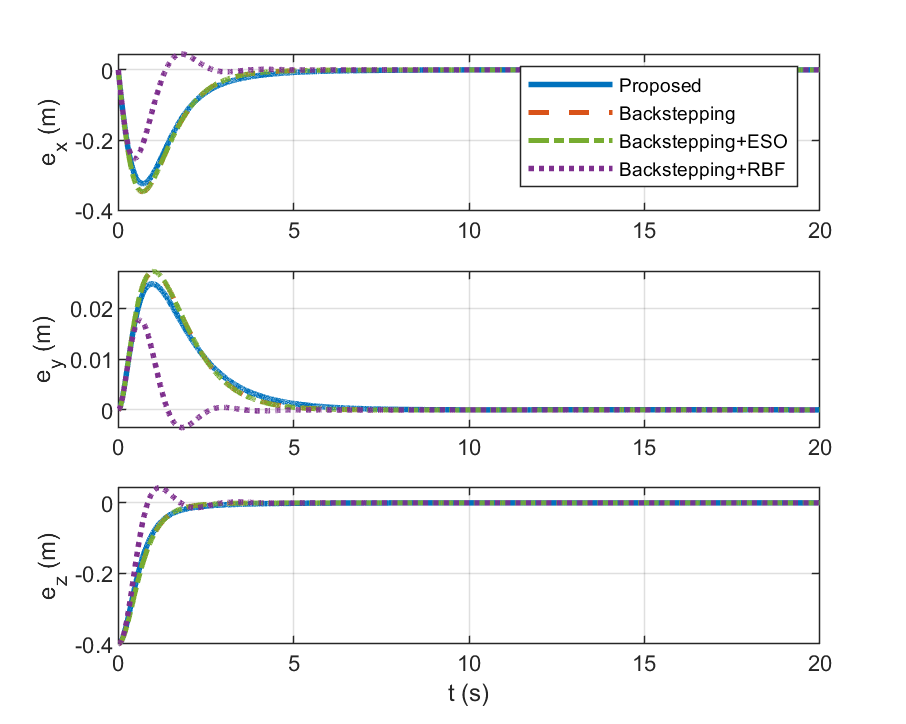
\includegraphics[width=\linewidth]{fig4a}\\
{\footnotesize (a) Position error}
\end{minipage}\hfill
\begin{minipage}[t]{0.48\textwidth}
\centering
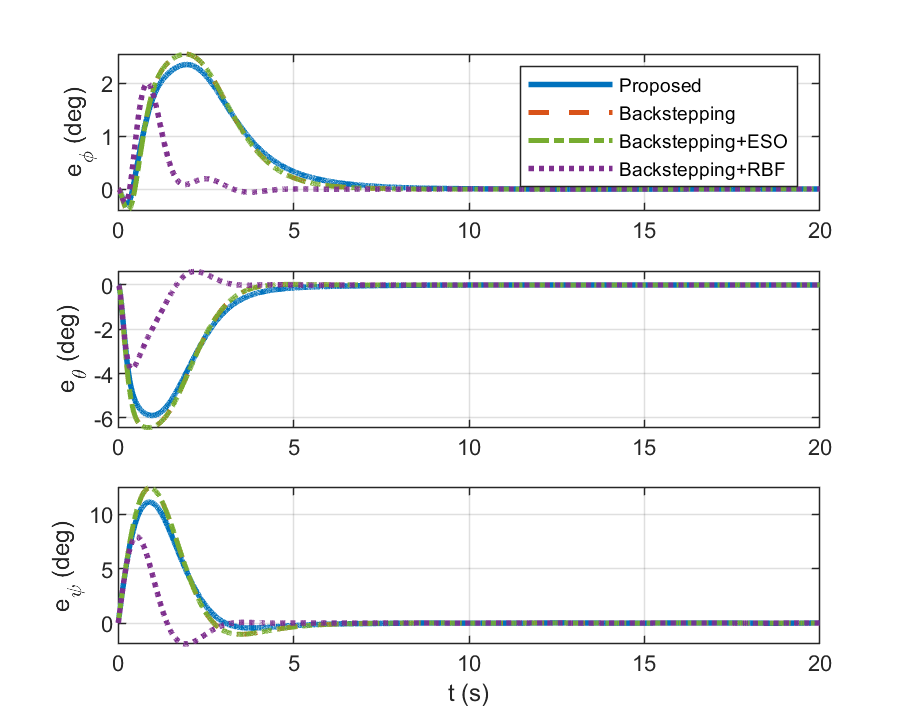
\includegraphics[width=\linewidth]{fig4b}\\
{\footnotesize (b) Attitude error}
\end{minipage}
\caption{Backstepping-family ablation without disturbance injection. All four
configurations reach the numerical floor, so this condition is shown for
completeness rather than as evidence of a module.}
\label{fig:ablation_nodist}
\end{figure}

\begin{figure}[t]
\centering
\begin{minipage}[t]{0.48\textwidth}
\centering
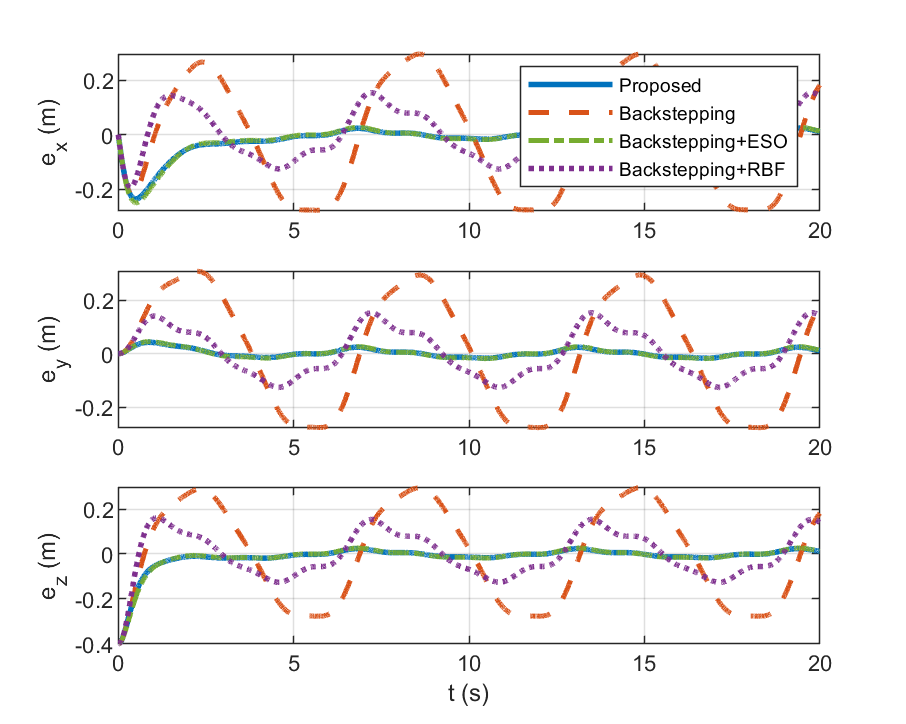
\includegraphics[width=\linewidth]{fig5a}\\
{\footnotesize (a) Position error}
\end{minipage}\hfill
\begin{minipage}[t]{0.48\textwidth}
\centering
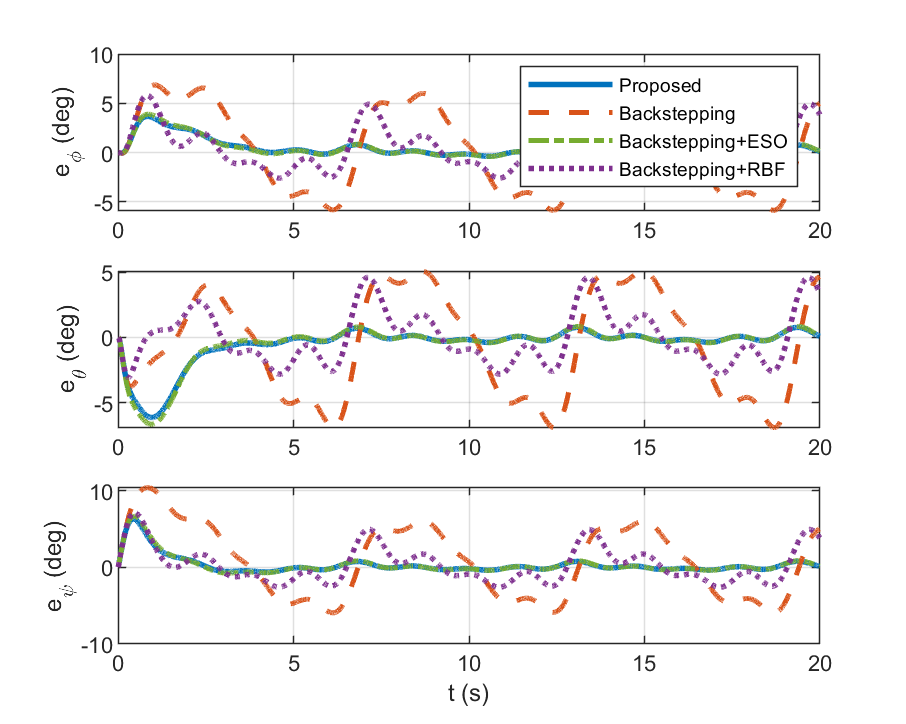
\includegraphics[width=\linewidth]{fig5b}\\
{\footnotesize (b) Attitude error}
\end{minipage}
\caption{Backstepping-family ablation with the periodic disturbance. The
observer removes most of the periodic error; the network adds a further
modest reduction.}
\label{fig:ablation_dist}
\end{figure}

\subsection*{Parameter Mismatch and Unmodeled Drag}

Tables~\ref{tab:mismatch} and~\ref{tab:drag} report the two robustness probes that use
the periodic disturbance. The nominal controller is kept unchanged in both
cases: the plant mass and inertia are scaled, or a quadratic drag force
$-\;c_d\|\mathbf{v}\|\mathbf{v}$ is added to the payload, which reaches about
$74\%$ of the payload weight at $c_d=12$.

The ESO-only configuration absorbs the mismatch: the error grows only from
$1.27\times10^{-2}$ to $3.99\times10^{-2}$~m while the plant is scaled from
$0.5$ to $1.5$ times the nominal value, a factor of three in the plant against
a factor of about three in the error. The composite-to-ESO ratio, however, stays
at $0.903$ across the whole sweep, and it also stays at $0.903$--$0.907$ as the
drag grows. A module that learned the mismatch or the velocity-dependent drag
would show a ratio that decreases with the severity of the perturbation; the
ratio does not move. The RBF term behaves instead like a roughly constant
scaling of the residual error.

\begin{table}[t]
\centering
\caption{Payload position RMS (m) under mass/inertia mismatch, periodic
disturbance. The last column is the composite-to-ESO ratio. Cells marked
``--'' were not run, because the plain backstepping case diverges far outside
the operating range of the comparison.}
\label{tab:mismatch}
\scriptsize
\setlength{\tabcolsep}{4pt}
\resizebox{\textwidth}{!}{%
\begin{tabular}{@{}lccccc@{}}
\hline
Scale & BS & BS+RBF & BS+ESO & BS+RBF+ESO & Ratio \\
\hline
$0.5$ & -- & $1.91\times10^{-1}$ & $1.27\times10^{-2}$ & $1.14\times10^{-2}$ & 0.903\\
$0.8$ & $2.68\times10^{-1}$ & $1.29\times10^{-1}$ & $2.07\times10^{-2}$ & $1.87\times10^{-2}$ & 0.903\\
$1.0$ & $3.38\times10^{-1}$ & $1.62\times10^{-1}$ & $2.62\times10^{-2}$ & $2.36\times10^{-2}$ & 0.903\\
$1.2$ & $5.39\times10^{-1}$ & $2.49\times10^{-1}$ & $3.16\times10^{-2}$ & $2.86\times10^{-2}$ & 0.903\\
$1.5$ & -- & $5.26\times10^{-1}$ & $3.99\times10^{-2}$ & $3.60\times10^{-2}$ & 0.903\\
\hline
\end{tabular}}
\end{table}

\begin{table}[t]
\centering
\caption{Payload position RMS (m) with an unmodeled quadratic drag,
periodic disturbance. The drag coefficient $c_d$ has units N\,s$^2$/m$^2$.}
\label{tab:drag}
\scriptsize
\setlength{\tabcolsep}{4pt}
\resizebox{\textwidth}{!}{%
\begin{tabular}{@{}lccccc@{}}
\hline
$c_d$ & BS & BS+RBF & BS+ESO & BS+RBF+ESO & Ratio \\
\hline
0  & $3.38\times10^{-1}$ & $1.62\times10^{-1}$ & $2.62\times10^{-2}$ & $2.36\times10^{-2}$ & 0.903\\
4  & $4.84\times10^{-1}$ & $2.13\times10^{-1}$ & $2.82\times10^{-2}$ & $2.55\times10^{-2}$ & 0.904\\
12 & $9.85\times10^{-1}$ & $6.57\times10^{-1}$ & $4.08\times10^{-2}$ & $3.70\times10^{-2}$ & 0.907\\
\hline
\end{tabular}}
\end{table}

\subsection*{Non-Periodic Disturbance}

The random-disturbance experiment replaces the periodic signal by
(\ref{eq:randomdist}) and repeats the four configurations on five fixed seeds.
All twenty runs completed, no metric was non-finite, no run exceeded the
$5$~m failure threshold, and no negative tension sample was recorded.

The ordering is the same as in the periodic case, and it is the same on every
seed rather than only on average: for each of the five seeds the composite is
better than ESO-only, ESO-only is better than RBF-only, and RBF-only is better
than plain backstepping. The magnitude of the RBF contribution shrinks: the
composite-to-ESO ratio is $0.943\pm0.011$, i.e.\ about $5.8\%$, against
$0.903$ under the periodic signal, while the observer still reduces the error
relative to plain backstepping by a factor of about seven.

These numbers must be compared with care. The two disturbance classes do not
have the same RMS: the periodic signal of (\ref{eq:dperiodic}) has an RMS of about
$2.15$~m/s$^2$ in translation, whereas the random one is normalised to
$1.0$~m/s$^2$. The absolute errors of the random runs are therefore lower for
all configurations, and the comparison is meaningful for the ordering and for
the ratio, not for absolute accuracy. Five seeds provide an indication of
dispersion, not statistical significance.

\begin{table}[t]
\centering
\caption{Non-periodic disturbance, five seeds: mean $\pm$ standard deviation
over the seeds, with the worst-case minimum tension and the total number of
failed runs.}
\label{tab:random}
\scriptsize
\setlength{\tabcolsep}{3pt}
\resizebox{\textwidth}{!}{%
\begin{tabular}{@{}lcccc@{}}
\hline
Configuration & Position RMS (m) & Position max (m) & Rotation RMS (rad) & Tension min (N)\\
\hline
Backstepping & $8.77\times10^{-2}\pm1.53\times10^{-2}$ & $1.41\times10^{-1}$ & $2.47\times10^{-2}\pm7.33\times10^{-3}$ & 3.518\\
Backstepping+RBF & $6.28\times10^{-2}\pm1.05\times10^{-2}$ & $1.04\times10^{-1}$ & $1.74\times10^{-2}\pm3.24\times10^{-3}$ & 3.319\\
Backstepping+ESO & $1.15\times10^{-2}\pm1.58\times10^{-3}$ & $1.88\times10^{-2}$ & $3.39\times10^{-3}\pm4.59\times10^{-4}$ & 3.213\\
Backstepping+RBF+ESO & $1.08\times10^{-2}\pm1.48\times10^{-3}$ & $1.78\times10^{-2}$ & $3.21\times10^{-3}\pm4.24\times10^{-4}$ & 3.204\\
\hline
\end{tabular}}
\end{table}

\begin{figure}[t]
\centering
\begin{minipage}[t]{0.48\textwidth}
\centering
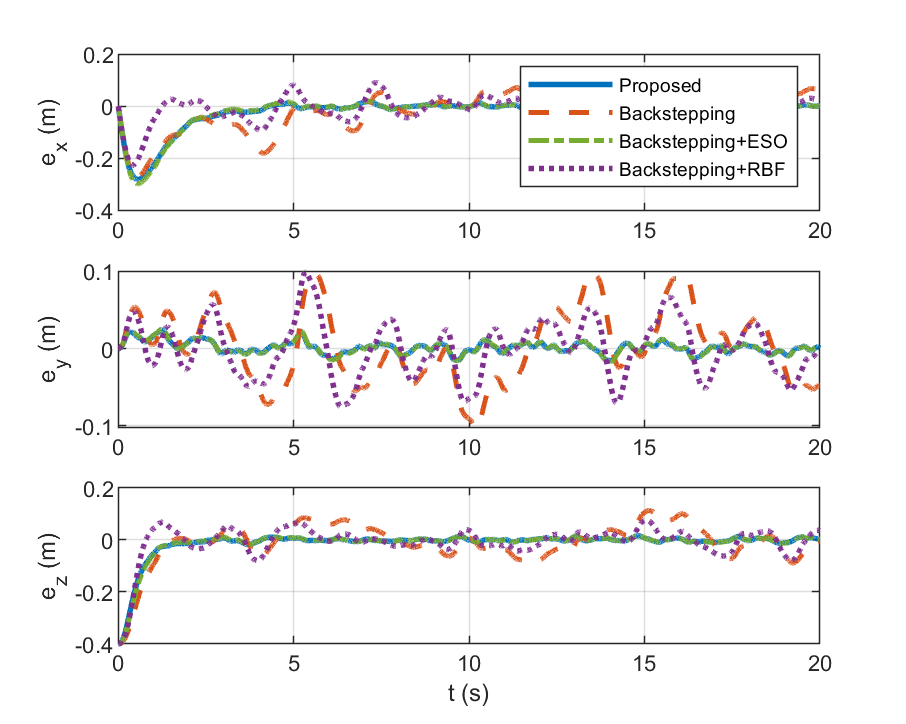
\includegraphics[width=\linewidth]{fig6a}\\
{\footnotesize (a) Position error}
\end{minipage}\hfill
\begin{minipage}[t]{0.48\textwidth}
\centering
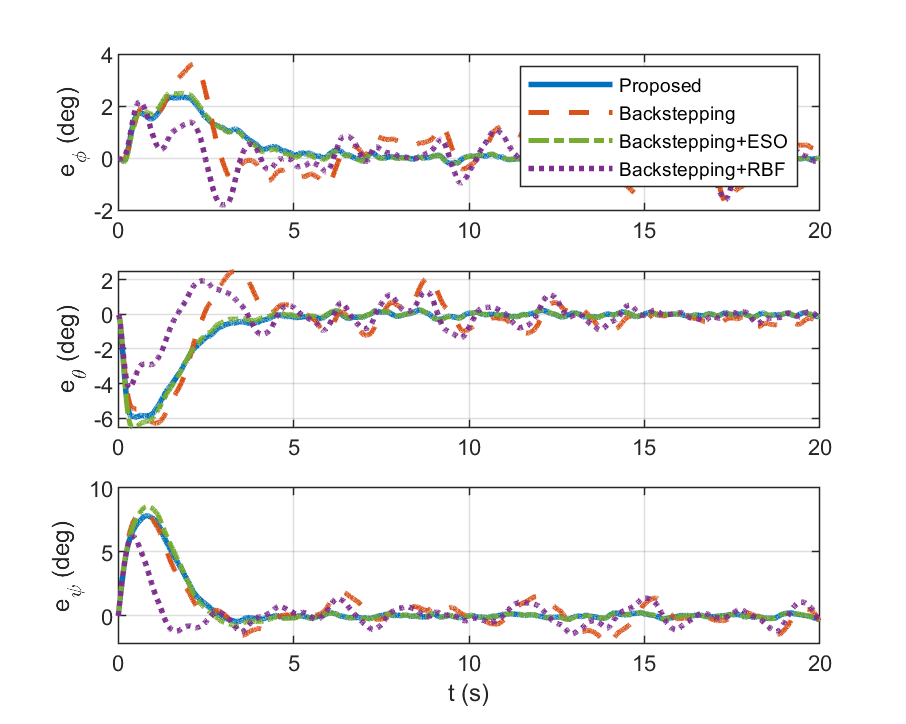
\includegraphics[width=\linewidth]{fig6b}\\
{\footnotesize (b) Attitude error}
\end{minipage}
\caption{Non-periodic band-limited disturbance, seed 101. The broadband
excitation produces a less regular error pattern than the periodic case, but
the ordering of the four configurations is unchanged.}
\label{fig:random}
\end{figure}

\subsection*{Interpretation}

Three statements are supported by the data. First, the observer is the
mechanism behind the large reduction: it lowers the payload error by an order
of magnitude under the periodic disturbance, by about seven times under the
random one, and it keeps the error within a factor of three when the plant is
scaled over a factor-of-three range. Second, the network contributes a
consistent but modest margin, $5.8$--$9.7\%$ depending on the disturbance
class, and the margin does not grow when the mismatch or the unmodeled
nonlinearity becomes more severe. Third, the ordering of the four
configurations is invariant across the disturbance classes tested, which is
what makes the ablation a usable comparison rather than an artefact of one
disturbance shape.

What the data do not support is equally important. They do not show that the
network identifies the unmodeled dynamics: a five-node static map of the
tracking error cannot represent a velocity-dependent drag, and the weight
norms remain small when the observer is active. They do not establish a
division of labour between learning and observation, and they do not
establish that the composite is the best choice in every condition; under no
disturbance the ESO-only configuration is in fact slightly worse than plain
backstepping, which is a numerical-floor effect rather than a performance
difference. Finally, five seeds and a single trajectory are not a statistical
study.

% ==================================================================
\section*{Limitations}
% ==================================================================

The evidence is bounded in several ways that the reader should weigh together.
The plant is a hierarchical reduced-order model: the payload is driven by the
allocated cable forces, but cable slackening, tension bounds, actuator
saturation, and aerodynamic interaction are not represented, so the reported
tensions are indicators of the reduced model rather than physical cable
tensions. The stability statement is conditional and covers the payload layer
with bounded implementation errors; it does not claim a full-system guarantee.
No hardware or hardware-in-the-loop experiment was performed. The comparison
is internal to the backstepping family: an external baseline such as a
sliding-mode or a non-neural adaptive backstepping controller would be needed
before claiming an advantage over the literature, and this revision does not
provide one. Computational cost is not reported here either; the controller is
evaluated in MATLAB on a desktop machine, which would not support a hard
real-time claim. Finally, the mismatch sweep scales mass and inertia together,
and the random experiment uses five seeds, so neither separates individual
parameter effects nor supports significance statements.

% ==================================================================
\section*{Conclusion}
% ==================================================================

This paper presented a payload-level RBF-ESO backstepping framework in which
the network output enters the observer prediction model, so that the observer
estimates the residual that remains after learning. The framework was evaluated
with one frozen parameter set in a backstepping-family ablation, a mass and
inertia mismatch sweep, an unmodeled quadratic drag, and a band-limited
non-periodic disturbance over five seeds.

The ablation bounds the role of each module. Observer-based compensation
accounts for most of the error reduction, by roughly an order of magnitude
under the periodic disturbance and by about seven times under the random one,
and it remains effective for mismatches up to $\pm50\%$ and for a drag reaching
about $74\%$ of the payload weight. The RBF term adds a consistent but modest
$5.8$--$9.7\%$, and the ratio does not respond to the severity of the mismatch
or of the unmodeled nonlinearity. The ordering of the four configurations is
preserved in every disturbance class tested. The contribution claimed here is
therefore the residual-consistent formulation, the conditional boundedness
analysis of the payload layer, and a quantitative statement of what each
module does and does not deliver, rather than a claim that the network learns
the unmodeled dynamics.

% ==================================================================
\section*{Simulation Parameters}
% ==================================================================

The physical, geometric, and numerical parameters are listed in
Table~\ref{tab:physical}; the single parameter set shared by all four configurations
is listed in Table~\ref{tab:gains}.

\begin{table}[t]
\centering
\caption{Physical, geometric, and numerical parameters.}
\label{tab:physical}
\scriptsize
\begin{tabular}{@{}p{0.30\textwidth}p{0.14\textwidth}p{0.46\textwidth}@{}}
\hline
Parameter & Symbol & Value\\
\hline
Number of quadrotors & $N$ & 3\\
Integration step and duration & $\Delta t$, $T_f$ & 0.001~s, 20~s\\
Quadrotor mass & $m_p$ & 2.0~kg for each UAV\\
Quadrotor inertia & $\mathbf{J}_p$ & $\mathrm{diag}(0.082,0.0845,0.1377)$~kg$\cdot$m$^2$\\
Payload mass & $m_L$ & 2.0~kg\\
Payload inertia & $\mathbf{J}_L$ & $\mathrm{diag}(0.113333,0.173333,0.273333)$~kg$\cdot$m$^2$\\
Payload dimensions & $L\times W\times H$ & $1.0\times0.8\times0.2$~m\\
Cable length & $l_i$ & 1.0~m for all three cables\\
Gravitational acceleration & $g$ & 9.81~m/s$^2$\\
Initial quadrotor positions & $\mathbf{p}_i(0)$ &
$[0.5,4.2,0]^{T}$, $[-0.5,4.6,0]^{T}$, $[-0.5,3.8,0]^{T}$\\
Initial payload position & $\mathbf{p}_L(0)$ & $[0,4.2,0.1]^{T}$\\
Attachment points & $\boldsymbol{\rho}_i$ &
$[0.5,0,0.1]^{T}$, $[-0.5,0.4,0.1]^{T}$, $[-0.5,-0.4,0.1]^{T}$\\
\hline
\end{tabular}
\end{table}

\begin{table}[t]
\centering
\caption{The single parameter set shared by all configurations and all
experiments. Only the compensation switches of Table~\ref{tab:ablation} change between
runs.}
\label{tab:gains}
\scriptsize
\setlength{\tabcolsep}{4pt}
\begin{tabular}{@{}p{0.26\textwidth}p{0.66\textwidth}@{}}
\hline
Group & Value\\
\hline
Payload backstepping gains &
$\mathbf{K}_{p1}=\mathbf{K}_{p0}=\mathrm{diag}(3,3,3)$, $\mathbf{K}_{p2}=\mathrm{diag}(1.5,1.5,1.5)$;
$\mathbf{K}_{\eta1}=\mathrm{diag}(3,3,3)$, $\mathbf{K}_{\eta2}=\mathrm{diag}(1.5,1.5,1.5)$\\
Allocation &
$K_{\Omega q}=[43.7,28.23,17.54]$, $K_q=[50,50.1,50]$, $\alpha_f=0.30$\\
UAV inner loop & backstepping thrust and moment controllers\\
RBF structure &
6 channels $\times$ 5 nodes; centres $(0,0),(\pm1,\pm1)$; width $b=0.8$;
initial weights $\hat{\boldsymbol{\theta}}_i(0)=\mathbf{0}$\\
RBF scaling &
translation $\mathrm{diag}(0.5\ \mathrm{m},0.5\ \mathrm{m/s})$;
attitude $\mathrm{diag}(0.10\ \mathrm{rad},0.50\ \mathrm{rad/s})$\\
RBF adaptation &
$\gamma_i=20$, $\sigma=0.05$, $\theta_{\max}=5$, compensation scale $1.0$\\
ESO &
$\omega_0=50$~rad/s, i.e.\ $\boldsymbol{\beta}=[3\omega_0,3\omega_0^{2},\omega_0^{3}]$ in each block;
compensation scale $1.0$; 18 states; previous-interval applied wrench\\
\hline
\end{tabular}
\end{table}

% ==================================================================
\begin{acks}
{This work was supported by the 2024 National Foreign Experts Project (Individual Category).}
\end{acks}

% ==================================================================
\section*{Declaration of conflicting interests}
% ==================================================================

The authors declare that there is no conflict of interest.

% ==================================================================
\begin{funding}
{This work was supported by the 2024 National Foreign Experts Project (Individual Category).}
\end{funding}

% ==================================================================
\begin{thebibliography}{99}
% ==================================================================

\bibitem[Bouabdallah and Siegwart(2005)]{bouabdallah2005}
Bouabdallah S and Siegwart R (2005) Backstepping and sliding-mode techniques applied to an
indoor micro quadrotor. In: \emph{Proceedings of the IEEE International Conference on Robotics
and Automation}. pp. 2247--2252. DOI:10.1109/ROBOT.2005.1570447.

\bibitem[Broomhead and Lowe(1988)]{broomhead1988}
Broomhead DS and Lowe D (1988) Multivariable functional interpolation and adaptive networks.
\emph{Complex Systems} 2: 321--355.

\bibitem[Estevez et al.(2024)]{estevez2024}
Estevez J, Garate G, Lopez-Guede JM and Larrea M (2024) Review of aerial transportation of
suspended-cable payloads with quadrotors. \emph{Drones} 8(2): 35. DOI:10.3390/drones8020035.

\bibitem[Fink et al.(2011)]{fink2011}
Fink J, Michael N, Kim S and Kumar V (2011) Planning and control for cooperative manipulation
and transportation with aerial robots. \emph{The International Journal of Robotics Research} 30(3):
324--334. DOI:10.1177/0278364910382803.

\bibitem[Gao(2003)]{gao2003}
Gao Z (2003) Scaling and bandwidth-parameterization based controller tuning.
In: \emph{Proceedings of the American Control Conference}, volume 6. pp. 4989--4996.
DOI:10.1109/ACC.2003.1242516.

\bibitem[Goodarzi et al.(2015)]{goodarzi2015}
Goodarzi FA, Lee D and Lee T (2015) Geometric control of a quadrotor UAV transporting a payload
connected by flexible cable. \emph{International Journal of Control, Automation and Systems} 13(6):
1486--1498. DOI:10.1007/s12555-014-0304-0.

\bibitem[Gu et al.(2022)]{gu2022}
Gu N, Wang D, Peng Z, Wang J and Han QL (2022) Disturbance observers and extended state
observers for marine vehicles: A survey. \emph{Control Engineering Practice} 123: 105158. DOI:
10.1016/j.conengprac.2022.105158.

\bibitem[Han(2009)]{han2009}
Han J (2009) From PID to active disturbance rejection control. \emph{IEEE Transactions on Industrial
Electronics} 56(3): 900--906. DOI:10.1109/TIE.2008.2011621.

\bibitem[Lee(2014)]{lee2014}
Lee T (2014) Geometric control of multiple quadrotor UAVs transporting a cable-suspended
rigid body. In: \emph{53rd IEEE Conference on Decision and Control}. pp. 6155--6160.
DOI:10.1109/CDC.2014.7040353.

\bibitem[Lee(2018)]{lee2018}
Lee T (2018) Geometric control of quadrotor UAVs transporting a cable-suspended rigid
body. \emph{IEEE Transactions on Control Systems Technology} 26(1): 255--264.
DOI:10.1109/TCST.2017.2656060.

\bibitem[Lee et al.(2013a)]{lee2013a}
Lee T, Leok M and McClamroch NH (2013a) Geometric control of multiple quadrotor UAVs
transporting a cable-suspended rigid body. \emph{IEEE Transactions on Control Systems Technology}
21(4): 1341--1356.

\bibitem[Lee et al.(2013b)]{lee2013b}
Lee T, Leok M and McClamroch NH (2013b) Nonlinear robust tracking control of a quadrotor
UAV on SE(3). \emph{Asian Journal of Control} 15(3): 391--408. DOI:10.1002/asjc.567.

\bibitem[Lee et al.(2013c)]{lee2013c}
Lee T, Sreenath K and Kumar V (2013c) Geometric control of cooperating multiple quadrotor
UAVs with a suspended payload. In: \emph{52nd IEEE Conference on Decision and Control}. pp.
5510--5515. DOI:10.1109/CDC.2013.6760757.

\bibitem[Madani and Benallegue(2008)]{madani2008}
Madani T and Benallegue A (2008) Adaptive control via backstepping technique and neural
networks of a quadrotor helicopter. In: \emph{IFAC Proceedings Volumes}, volume 41. pp. 6513--
6518. DOI:10.3182/20080706-5-KR-1001.01098.

\bibitem[Mado\'nski and Herman(2015)]{madonski2015}
Mado\'nski R and Herman P (2015) Survey on methods of increasing the efficiency of extended state
observers. \emph{ISA Transactions} 56: 18--27. DOI:10.1016/j.isatra.2014.11.008.

\bibitem[Park and Sandberg(1991)]{park1991}
Park J and Sandberg IW (1991) Universal approximation using radial-basis-function networks.
\emph{Neural Computation} 3(2): 246--257. DOI:10.1162/neco.1991.3.2.246.

\bibitem[Sanner and Slotine(1992)]{sanner1992}
Sanner RM and Slotine JJE (1992) Gaussian networks for direct adaptive control.
\emph{IEEE Transactions on Neural Networks} 3(6): 837--863. DOI:10.1109/72.165588.

\bibitem[Shen and Xu(2021)]{shen2021}
Shen S and Xu J (2021) Adaptive neural network-based active disturbance rejection flight
control of an unmanned helicopter. \emph{Aerospace Science and Technology} 119: 107062. DOI:
10.1016/j.ast.2021.107062.

\bibitem[Sreenath et al.(2013)]{sreenath2013}
Sreenath K, Michael N and Kumar V (2013) Trajectory generation and control of a quadrotor
with a cable-suspended load--a differentially-flat hybrid system.
In: \emph{Proceedings of the
IEEE International Conference on Robotics and Automation}. pp. 4888--4895.
DOI:10.1109/ICRA.2013.6631275.

\bibitem[Thanh et al.(2022)]{thanh2022}
Thanh HLNN, Huynh TT, Vu MT, Mung NX, Tran HS, Kim SK, Vu TL and Nguyen NV (2022)
Quadcopter UAVs extended states/disturbance observer-based nonlinear robust backstepping
control under uncertainties and disturbances. \emph{Sensors} 22(14): 5082. DOI:10.3390/s22145082.

\bibitem[Wang et al.(2022)]{wang2022}
Wang Z et al. (2022) Adaptive-based linear active disturbance rejection attitude control for a
quadrotor UAV with external disturbances. \emph{Transactions of the Institute of Measurement and
Control} DOI:10.1177/01423312211031781.

\end{thebibliography}

\end{document}


